\documentclass[preprint,12pt]{elsarticle}

%% Use the option review to obtain double line spacing
%% \documentclass[preprint,review,12pt]{elsarticle}

%% Use the options 1p,twocolumn; 3p; 3p,twocolumn; 5p; or 5p,twocolumn
%% for a journal layout:
%% \documentclass[final,1p,times]{elsarticle}
%% \documentclass[final,1p,times,twocolumn]{elsarticle}
%% \documentclass[final,3p,times]{elsarticle}
%% \documentclass[final,3p,times,twocolumn]{elsarticle}
%% \documentclass[final,5p,times]{elsarticle}
%% \documentclass[final,5p,times,twocolumn]{elsarticle}

%% The amssymb package provides various useful mathematical symbols
\usepackage{amssymb}
%% The amsthm package provides extended theorem environments
\usepackage{amsthm}

\newtheorem{theorem}{Theorem}[section]
\newtheorem{example}{Example}[section]
\newtheorem{definition}{Definition}[section]
\newtheorem{proposition}{Proposition}[section]

\usepackage{pgfplots}
\pgfplotsset{width=10cm,compat=1.13}
\usepgfplotslibrary{groupplots}

%% The lineno packages adds line numbers. Start line numbering with
%% \begin{linenumbers}, end it with \end{linenumbers}. Or switch it on
%% for the whole article with \linenumbers.
\usepackage{lineno}

\usepackage{hyperref}
\hypersetup{pdfauthor={Name}} % avoid warning messages from hyperref package in LaTex

%%%%%%%%%%%%%%%%%%%%%%%%%%%%%%%%%%%%%%%%%%%%%%%%%%%%%%%%%%%%
%% Drawing
%%%%%%%%%%%%%%%%%%%%%%%%%%%%%%%%%%%%%%%%%%%%%%%%%%%%%%%%%%%%
\usepackage{tikz}
\usepackage{amsfonts}

% drawing automa
\usetikzlibrary{positioning,automata}

% for captions in figures
\usepackage[labelformat=simple]{subcaption}
\renewcommand\thesubfigure{(\alph{subfigure})}

\usepackage{booktabs}

% table row numbers
\newcounter{rownumber}
\newcommand\rownb{\stepcounter{rownumber}\arabic{rownumber}}

\newcommand{\vangiang}[1]{\textcolor{magenta}{#1}}
\newcommand{\belaid}[1]{\textcolor{blue}{#1}}
\newcommand{\sylvain}[1]{\textcolor{teal}{#1}}

\newcommand{\revBelaid}[1]{\textcolor{red}{#1}}

\usepackage{amsmath}
\newcommand{\IN}{\mathit{IN}}
\DeclareMathOperator{\pred}{pred}
\let\succ\relax
\DeclareMathOperator{\succ}{succ}

\journal{Theoretical Computer Science}

\begin{document}

\begin{frontmatter}

%% Title, authors and addresses

%% use the tnoteref command within \title for footnotes;
%% use the tnotetext command for theassociated footnote;
%% use the fnref command within \author or \address for footnotes;
%% use the fntext command for theassociated footnote;
%% use the corref command within \author for corresponding author footnotes;
%% use the cortext command for theassociated footnote;
%% use the ead command for the email address,
%% and the form \ead[url] for the home page:
%% \title{Title\tnoteref{label1}}
%% \tnotetext[label1]{}
%% \author{Name\corref{cor1}\fnref{label2}}
%% \ead{email address}
%% \ead[url]{home page}
%% \fntext[label2]{}
%% \cortext[cor1]{}
%% \affiliation{organization={},
%%             addressline={},
%%             city={},
%%             postcode={},
%%             state={},
%%             country={}}
%% \fntext[label3]{}

\title{Trap spaces of Boolean networks are conflict-free siphons of their Petri net encoding}

%% use optional labels to link authors explicitly to addresses:
%% \author[label1,label2]{}
%% \affiliation[label1]{organization={},
%%             addressline={},
%%             city={},
%%             postcode={},
%%             state={},
%%             country={}}
%%
%% \affiliation[label2]{organization={},
%%             addressline={},
%%             city={},
%%             postcode={},
%%             state={},
%%             country={}}

\author{Van-Giang Trinh\fnref{1}}
\ead{trinh.van-giang@lis-lab.fr}

\author{Belaid Benhamou\fnref{1}}
\ead{belaid.benhamou@lis-lab.fr}

\affiliation[1]{organization={LIS, Aix-Marseille University},%Department and Organization
            %addressline={},
            city={Marseille},
            %postcode={},
            %state={},
            country={France}}

\author{Sylvain Soliman\corref{cor1}\fnref{2}}
\ead{Sylvain.Soliman@inria.fr}

\affiliation[2]{organization={Lifeware team, Inria Saclay center},%Department and Organization
            %addressline={},
            city={Palaiseau},
            %postcode={},
            %state={},
            country={France}}

\cortext[cor1]{Corresponding author.}

\begin{abstract}
%% Text of abstract

Boolean network modeling of gene regulation but also of post-trans\-criptomic systems has proven over the years that it can bring powerful analyses and corresponding insight to the many cases where precise biological data is not sufficiently available to build a detailed quantitative model.
%This is even more true for very large models where such data is frequently missing and led to a constant increase in size of logical models \emph{à la} Thomas.
Besides simulation, the analysis of such models is mostly based on attractor computation, since those correspond roughly to observable biological \emph{phenotypes}.
The recent use of trap spaces made a real breakthrough in that field allowing to consider medium-sized models that used to be out of reach.
However, with the continuing increase in model size and complexity of Boolean update functions, the state-of-the-art computation of minimal trap spaces based on \emph{prime-implicants} shows its limits due to the difficulty of the prime-implicant computation.

In this article we explore and prove for the first time a connection between trap spaces of a general Boolean network and siphons of its Petri net encoding.
Besides important theoretical applications in studying properties of trap spaces, the connection enables us to propose an alternative approach to compute minimal trap spaces, and hence complex attractors, of a general Boolean network.
It replaces the need for prime-implicants by a completely different technique, namely the enumeration of maximal siphons in the Petri net encoding of the original model.
We then demonstrate its efficiency and compare it to the state-of-the-art methods on a large collection of real-world and randomly generated models.

\end{abstract}

%%Graphical abstract
% \begin{graphicalabstract}
% %\includegraphics{grabs}
% \end{graphicalabstract}

%%Research highlights
% \begin{highlights}
% \item Research highlight 1
% \item Research highlight 2
% \end{highlights}

\begin{keyword}
%% keywords here, in the form: keyword \sep keyword

%% PACS codes here, in the form: \PACS code \sep code

%% MSC codes here, in the form: \MSC code \sep code
%% or \MSC[2008] code \sep code 2000 is the default

Logical model \sep Boolean network \sep Trap space \sep Attractor computation \sep Petri net \sep Siphon \sep Systems biology
\end{keyword}

\end{frontmatter}

\linenumbers%

%% main text
\section{Introduction}

From the observation that the transcriptional regulation behaved in a sigmoid step-like way, came the original idea to represent models of gene regulation as discrete event systems.
Those gene regulation networks use thresholds or equivalently logical functions to represent the different regulations~\cite{glass1973logical,thomas1973boolean,thomas1990biological,thomas1991regulatory}.

Boolean modeling made available some powerful analyses and corresponding insight for gene regulation models.
Then, over the years, its use increased even for modelling post-transcriptional mechanisms, supported by the many cases where precise biological data was not sufficiently available to build a detailed quantitative model~\cite{wang2012boolean}.
This lack of data is more frequent for large and very large models, which led to a steady increase in the size of logical models \emph{à la} Thomas~\cite{aghamiri2020automated}.
The main analysis tool for such models is the computation of its fixed and periodic attractors, since those correspond roughly to observable biological \emph{phenotypes}.
The recent use of trap spaces~\cite{klarner2015computing} made a real breakthrough in that field allowing to consider medium-sized models that used to be out of reach and for which only simulation was available.
However, with the most recent models both being quite large and using rather complex update functions, the state-of-the-art computation of minimal trap spaces based on \emph{prime-implicants} shows its limits.
More specifically, the number of prime implicants of a Boolean function is in general exponential in the number of input nodes of this function~\cite{klarner2015computing}.
Moreover, the computation of prime implicants is a demanding task, especially for complex Boolean functions.

It is worth noting that the recent method presented in~\cite{DBLP:conf/ictai/ChevalierFPZ19} for computing minimal trap spaces avoids the prime-implicant computation by relying on the \emph{most-permissive} semantics of Boolean networks.
This method has been implemented in the tool \texttt{mpbn}\footnote{\url{https://github.com/bnediction/mpbn}} demonstrated in~\cite{Paulev2020} for handling medium-sized models from the literature and very large synthetic models (up to 100,000 nodes).
However, this method is only applicable for \emph{locally-monotonic} Boolean networks, whereas the prime-implicants based method~\cite{klarner2015computing} is applicable for \emph{general} Boolean networks (i.e., including both locally-monotonic and non-locally-monotonic ones).
In addition, the \texttt{bioLQM} platform also provides another method using Binary Decision Diagrams (BDDs) in \url{http://colomoto.org/biolqm/doc/tools-trapspace.html}.
This method avoids the prime-implicant computation as it characterizes the set of generic trap spaces of a Boolean network by a BDD, then filters this set to get the set of all minimal trap spaces.
By this approach, it requires the computation of all solutions, whereas the methods~\cite{klarner2015computing,Paulev2020} based on Answer Set Programming (ASP) can start enumerating them as they are found.
Moreover, the main issue with the BDD-based method is that the number of generic trap spaces of a Boolean network may be extremely larger than its number of minimal trap spaces.
This issue limits the efficiency of the BDD-based method.
The study~\cite{DBLP:journals/tcs/NoualRS13} highlights the need for non-locally-monotonic Boolean networks in both biological and theoretical aspects.
Hence, it is still necessary to develop efficient methods for computing minimal trap spaces of large-scale general Boolean networks.

Petri nets were introduced in the 60s as simple formalism for describing and analyzing information-processing systems that are characterized as being concurrent, asynchronous, non-deterministic and possibly distributed~\cite{peterson1981petri,Murata1989}.
The use of Petri nets for representing biochemical reaction systems, by mapping molecular species to places and reactions to transitions, hinted at already in~\cite{peterson1981petri,Murata1989} was used more thoroughly quite late in~\cite{reddy1993petri}, together with some Petri net concepts and tools for the analysis of metabolic networks.
Siphons are such a concept, but they have not been used a lot for the study of biochemical systems~\cite{zevedei2003topological,blatke2015biomodel} even if the practical cost of computing their minimal/maximal elements appear much more manageable than the theoretical complexity would indicate~\cite{oanea2010new,nabli2016enumerating}.

In this article we explore and prove for the first time a connection between trap spaces of a general Boolean network and siphons of its Petri net encoding.
Not only having important theoretical applications in studying properties of trap spaces in Boolean networks, the connection has important practical applications in the trap space computation.
Specifically, based on the connection, we propose an alternative approach to compute minimal trap spaces, and hence complex attractors, of a general Boolean network.
It replaces the need for prime-implicants by a completely different technique, namely the enumeration of maximal siphons in the Petri net encoding of the original model.
We then demonstrate its efficiency and compare it to the state-of-the-art methods for computing minimal trap spaces of Boolean networks on many real-world models from various sources in the literature and on randomly generated models.

%After recalling several technical preliminaries (Section~\ref{sec:Preliminaries}), we expose the concrete need for such a method and detail its implementation using Answer Set Programming (Section~\ref{sec:Computation}).

%All models used for evaluation and the implementation of the presented method are available at \url{https://github.com/soli/trap-spaces-as-siphons} and executable as a CoLoMoTo docker image.

% Mention the extensions for the journal version
Herein we revise and extend our previous work in~\cite{DBLP:conf/cmsb/TrinhBHS22} as follows.
First, more formal definitions are given and the existing proofs are made more detailed.
In particular, an updated proof provides another way to prove the independence of trap spaces of a Boolean network with respect to its update scheme, which was originally proved in~\cite{klarner2015computing}.
Second, we showcase a theoretical application of the connection between trap spaces in Boolean networks and conflict-free siphons in Petri nets.
Third, beyond the proposed ASP method implementing the alternative approach~\cite{DBLP:conf/cmsb/TrinhBHS22}, we propose several other possible methods for computing minimal trap spaces using Maximum Satisfiability (MaxSAT), Constraint Programming (CP), and Integer Linear Programming (ILP).
Fourth, we discuss in detail how to compute several special types of trap spaces in a Boolean network.
Besides minimal trap spaces, these special types also play crucial roles in analyzing and controlling Boolean networks~\cite{Rozum2021}.
%Fifth, we present the idea for using our Petri net approach to handle the problem of inconsistent and incomplete data in modeling biological systems.
Fifth, regarding the implementation, we have developed a new converter that directly reads a \texttt{.bnet} file and builds the Petri net encoding, instead of using the \texttt{PNML} conversion of \texttt{bioLQM}~\cite{DBLP:conf/cmsb/TrinhBHS22}.
Finally, we conduct a more extensive benchmark on more real-world models from various sources and randomly generated models to evaluate all the proposed methods (the benchmark conducted in~\cite{DBLP:conf/cmsb/TrinhBHS22} considers only a few dozens of representative real-world models), therefore obtaining more comprehensive insights.

%%% Paper structure %%%
The rest of this paper is organized as follows: Section~\ref{sec:Preliminaries} recalls the basic concepts including Boolean networks, attractors, trap spaces, Petri nets, and siphons.
Section~\ref{sec:Main_finding} presents the main finding, the connection between trap spaces in Boolean networks and siphons in Petri nets.
Section~\ref{sec:Computation} presents the alternative approach for computing minimal trap spaces and the four possible methods implementing it.
%Section~\ref{sec:incomplete-data} presents the idea to deal with problem of inconsistent and incomplete data.
Section~\ref{sec:case_study} shows an important biological case study showing the applicability of the new approach.
Section~\ref{sec:eval} reports the experimental results for evaluating the efficiency of the proposed methods.
Finally, Section~\ref{sec:Conclusion} concludes the paper and draws future work.

\section{Preliminaries}%
\label{sec:Preliminaries}

We shall briefly recall here some preliminaries on Boolean networks related to trap spaces and Petri nets.
%In the case of multi-level logical models, an encoding into a Boolean network is always possible~\cite{Didier2011}.
%\vangiang{Remove this statement because there is not sure if the encoded Boolean network preserves the trap spaces of the original multi-level logical model.}

\subsection{Boolean networks}

\begin{definition}%
\label{def:BN}

  A Boolean Network (BN) is a pair \(\mathcal{N} = (V, F)\) where:
  \begin{itemize}
    \item \(V = \{v_1, \dots, v_n\}\) is the set of nodes.
    We use \(v_i\) to denote both the node \(v_i\) and its associated Boolean variable.

    \item \(F = \{f_1, \dots, f_n\}\) is the set of update functions.
    Each function \(f_i\) is associated with node \(v_i\) and satisfies \(f_i \colon \mathbb{B}^{\vert \IN(v_i)\vert} \mapsto \mathbb{B}\) where \(\mathbb{B} = \{0, 1\}\) and \(\IN(v_i)\) denotes the set of input nodes of \(v_i\).
    Note that a node \(v_i \in V\) is called a \emph{source} node if and only if \(f_{i} = v_i\).
  \end{itemize}

\end{definition}

A Boolean function is \emph{locally-monotonic} if it can be represented by a formula in disjunctive normal form in which all occurrences of any given literal are either negated or non-negated~\cite{Paulev2020}.
A Boolean network is said to be locally-monotonic if all its Boolean functions are locally-monotonic.
Otherwise, this model is said to be non-locally-monotonic.

A state \(v \in \mathbb{B}^{n}\) is as a mapping \(v \colon V \mapsto \mathbb{B}\) that assigns either 0 (inactive) or 1 (active) to each node.
We denote the set of all possible states of a Boolean network \(\mathcal{N}\) by \(\mathcal{S}_{\mathcal{N}} = \mathbb{B}^n\).
At each time step \(t\), node \(v_i\) can, depending on the update scheme, update its state by
\[v_i(t + 1) =
  \begin{cases}
    &f_i(v(t))\\
    \text{or} &v_i(t)
  \end{cases}
\]
where \(v(t)\) (resp. \(v_i(t)\)) is the state of \(\mathcal{N}\) (resp. the state of node \(v_i\)) at time \(t\). % and \(v_i(t + 1)\) is the state of node \(v_i\) at time \(t + 1\).
Note that for simplicity, we write \(f_i(v(t))\) even if \(\IN(v_i) \subsetneq V\) (i.e., \(\IN(v_i)\) does not contain some nodes of \(V\)).
An update scheme of a Boolean network specifies which nodes update their states, as defined above, through time evolution~\cite{thomas1991regulatory}.
Following the update scheme, the Boolean network transits from a state to another state (possibly identical).
This transition is called the \emph{state transition} and denoted by \(\rightarrow \subseteq \mathcal{S}_{\mathcal{N}} \times \mathcal{S}_{\mathcal{N}}\).
Then the dynamics of \(\mathcal{N}\) is captured by the directed graph \((\mathcal{S}_{\mathcal{N}}, \rightarrow)\) called the State Transition Graph (STG).
There are many different update schemes, but the two main types~\cite{thomas1991regulatory} are: \emph{synchronous}, where all the nodes are update simultaneously, and \emph{fully asynchronous}, where only one node is selected non-deterministically to be updated.

\subsection{Traps spaces}

We recall here some definitions from~\cite{klarner2015computing} for the introduction of \emph{trap spaces}.
Minimal trap spaces prove to be a very good approximation of the attractors of a Boolean network under asynchronous update schemes and have become the \emph{de facto} standard way to analyze models of a few tens of \emph{genes}~\cite{klarner2017pyboolnet,cifuentes2020control}.

A non-empty set \(T \subseteq \mathcal{S}_{\mathcal{N}}\) is a trap set with respect to \(\rightarrow\) if for every \(x \in T\) and \(y \in S\) with \(x \rightarrow y\) it holds that \(y \in T\)~\cite{klarner2015computing}.
An attractor of \(\mathcal{N}\) with respect to \(\rightarrow\) can be defined as an inclusion-wise minimal trap set of \((\mathcal{S}_{\mathcal{N}}, \rightarrow)\).
An attractor can be also seen as a terminal strongly connected component of \((\mathcal{S}_{\mathcal{N}}, \rightarrow)\)~\cite{chatain2014characterization}.
An attractor of size 1 is called a fixed point, otherwise it is called a cyclic or complex attractor~\cite{klarner2015computing}.

A subspace \(m\) of a Boolean network \(\mathcal{N} = (V, F)\) is a mapping \(m \colon V \mapsto \mathbb{B} \cup \{\star\}\).
\(m(v_i) \in \mathbb{B}\) means that the value of \(v_i\) is fixed in \(m\) and \(v_i\) is called a \emph{fixed} variable.
\(m(v_i) \in \star\) means that the value of \(v_i\) is free in \(m\) and \(v_i\) is called a \emph{free} variable.
We denote \(D_m\) the set of all fixed variables of \(m\).
A subspace \(m\) is equivalent to a set of states:
\[
\mathcal{S}_{\mathcal{N}}[m] := \{s \in \mathcal{S}_{\mathcal{N}} \mid \forall v \in D_m \colon s(v) = m(v)\}.
\] For example, \(m = \star\star1\) (for simplicity, we shall write subspaces likes states as a sequence of values) means that \(D_m = \{v_3\}, m(v_3) = 1\), and it is equivalent to the set of states \(\{001, 011, 101, 111\}\).
We denote \(\mathcal{S}_{\mathcal{N}}^{\star} = (\mathbb{B} \cup \{\star\})^n\) the set of all possible subspaces of \(\mathcal{N}\).
Note that \(\left\vert\mathcal{S}_{\mathcal{N}}^{\star}\right\vert = 3^n\) and \(S_{\mathcal{N}} \subset \mathcal{S}_{\mathcal{N}}^{\star}\)~\cite{klarner2015computing}.

A \emph{trap space} is defined as a subspace that is also a trap set.
It is noted that trap spaces of a Boolean network are independent of the update scheme of this model~\cite{klarner2015computing}.
Then, we define a partial order \(<\) on \(\mathcal{S}_{\mathcal{N}}^{\star}\) as: \(m < m'\) if and only if \(\mathcal{S}_{\mathcal{N}}[m] \subseteq \mathcal{S}_{\mathcal{N}}[m']\) and \(\mathcal{S}_{\mathcal{N}}[m] \neq \mathcal{S}_{\mathcal{N}}[m']\).
Consequently, a trap space \(m\) is minimal if and only if there is no trap space \(m' \in \mathcal{S}_{\mathcal{N}}^{\star}\) such that \(m' < m\).

For example, let us consider the Boolean network shown in Example~\ref{example:BN}.
Figure~\ref{fig:stg} shows the dynamics of this model under the fully asynchronous update (i.e., only one node is updated at each time step).
The model has all two trap spaces, \(m_1 = 11\) and \(m_2 = \star\star\).
Since \(m_1 < m_2\), \(m_1\) is the only minimal trap space of the Boolean network.

\begin{example}
We give a Boolean network \(\mathcal{N} = (V, F)\), where \(V = (x_1, x_2)\) and \(F = (f_1, f_2)\) with \(f_1 = (x_1 \land x_2) \lor (\neg x_1 \land \neg x_2), f_2 = (x_1 \land x_2) \lor (\neg x_1 \land \neg x_2)\). Herein, \(\land\), \(\lor\), and \(\neg\) denote the \revBelaid{logical conjunction, disjunction, and negation operators}, respectively.\label{example:BN}
\end{example}

\begin{figure}[!htb]
\centering
\begin{subfigure}[b]{0.3\textwidth}
\centering
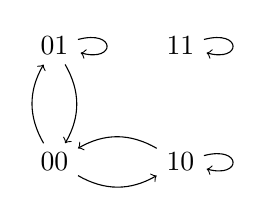
\begin{tikzpicture}[node distance=1cm and 1cm, every node/.style={scale=1.0}]
   \node[] (0) [] {00};
   \node[] (1) [above=of 0] {01};
   \node[] (2) [right=of 0] {10};
   \node[] (3) [above=of 2] {11};

   \draw[->] (0) edge [bend left] (1);
   \draw[->] (0) edge [bend right] (2);

   \draw[->] (1) edge [bend left] (0);
   \draw[->] (1) edge [loop right] (1);

   \draw[->] (2) edge [bend right] (0);
   \draw[->] (2) edge [loop right] (2);

   \draw[->] (3) edge [loop right] (3);
\end{tikzpicture}
\caption{State transition graph, under the fully asynchronous update.}%
\label{fig:stg}
\end{subfigure}\hfill%
\begin{subfigure}[b]{0.6\textwidth}
\centering
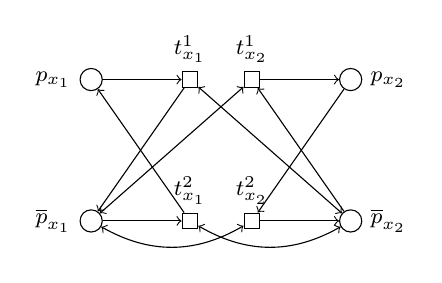
\begin{tikzpicture}[node distance=1cm and 1cm, every node/.style={scale=1.0}]\footnotesize
  \node[circle,draw,label=left:$p_{x_1}$] (x1) {};
  \node[circle,draw,label=left:$\overline{p}_{x_1}$] (nx1) [below=of x1, yshift=-0.5cm] {};

  \node[circle,draw,label=right:$p_{x_2}$] (x2) [right=of x1, xshift=2.0cm] {};
  \node[circle,draw,label=right:$\overline{p}_{x_2}$] (nx2) [below=of x2, yshift=-0.5cm] {};

  \node[rectangle,draw,label=above:$t^1_{x_1}$] (t1x1) [right=of x1] {};
  \node[rectangle,draw,label=above:$t^2_{x_1}$] (t2x1) [right=of nx1] {};

  \node[rectangle,draw,label=above:$t^1_{x_2}$] (t1x2) [left=of x2] {};
  \node[rectangle,draw,label=above:$t^2_{x_2}$] (t2x2) [left=of nx2] {};

  \draw[->] (x1) -- (t1x1);
  \draw[->] (t1x1) -- (nx1);
  \draw[<->] (t1x1) -- (nx2);

  \draw[->] (nx1) -- (t2x1);
  \draw[->] (t2x1) -- (x1);
  \draw[<->] (t2x1) edge [bend right] (nx2);

  \draw[->] (x2) -- (t2x2);
  \draw[->] (t2x2) -- (nx2);
  \draw[<->] (t2x2) edge [bend left] (nx1);

  \draw[->] (nx2) -- (t1x2);
  \draw[->] (t1x2) -- (x2);
  \draw[<->] (t1x2) -- (nx1);
\end{tikzpicture}
\caption{Petri net encoding of the model. Circles denote places, whereas rectangles denote transitions.}%
\label{fig:PN}
\end{subfigure}%
\caption{Dynamics and encoding of the Boolean network of Example~\ref{example:BN}.}%
\label{fig:stg_and_PN}
\end{figure}

\subsection{Petri net encoding of Boolean networks}%
\label{sec:encoding}

\begin{definition}

  A \emph{Petri net} is a weighted bipartite directed graph \((P, T, W)\),
  where \(P\) is a non-empty finite set of vertices called \emph{places},
  \(T\) is a non-empty finite set of vertices called \emph{transitions},
  \(P \cap T = \emptyset\),
  and \(W : (P \times T) \cup (T \times P) \mapsto \mathbb{N} \) is a weight function attached to the arcs.

\end{definition}
A \emph{marking} for a Petri net is a mapping \(m : P \mapsto \mathbb{N}\) that assigns a number of tokens to each place.
A place \(p\) is marked by a marking \(m\) if and only if \(m(p) > 0\).
Marking \(m\) can be seen as a subset of \(P\) that contains all marked places by \(m\).
We shall write \(\pred(x)\) (resp.\ \(\succ(x)\)) to represent the set of vertices that have a (non-zero weighted) arc leading to (resp.\ coming from) \(x\).
In this work, we consider a class of Petri nets called 1-safe Petri nets where every place has at most 1 token and all arcs are of weight 1.
In this case, weights are implicitly omitted in the arcs of a Petri net.
Then, a transition \(t \in T\) is \emph{enabled} at a marking \(m\) if and only if \(\pred(t) \subseteq m\).
A marking \(m\) is called a deadlock if there are no enabled transitions at \(m\).
The firing of \(t\) leads to a new marking \(m'\) specified by \(m' = (m \backslash \pred(t)) \cup \succ(t)\).
Note that when multiple transitions are enabled, we need to embed one firing scheme (similar to the update scheme of a Boolean network) to the Petri net.
The classical firing scheme is that only one of the enabled transition is non-deterministically chosen to fire~\cite{Murata1989}.

The link between Boolean networks \emph{à la} Thomas and Petri nets was originally established in~\cite{chaouiya2004qualitative} in order to make available formal methods like model-checking for the analysis of such systems.
The basic encoding into 1-safe (i.e., never more than one token in each place) nets only holds for purely Boolean networks but was later extended to multivalued logical models in two ways, either in~\cite{chaouiya2011petri} with non 1-safe Petri nets or more recently in~\cite{chatain2014characterization} with 1-safe nets but many more places.

Since our study is focused on Boolean networks, we briefly recall the original encoding here.
Its basis is that every node (\emph{gene}) \(v\) of the original model \(\mathcal{N} = (V, F)\) is represented by two separate places (\(p_v\) and \(\overline{p}_v\)), corresponding to its two states, active, and inactive, respectively.
Each conjunct of the logical function that activates the \emph{gene} will lead to a transition \(t\), consuming the inactive place (i.e., a directional arc from \(\overline{p}_v\) to \(t\)), producing the active place (i.e., a directional arc from \(t\) to \(p_v\)), and with all other literals both consumed and produced (i.e., a bidirectional arc).
And conversely for the inactivation.
Let \(s\) be a state of the Boolean network and \(m_s\) be its corresponding marking in the encoded Petri net.
It holds that \(\forall v \in V\), \(s(v) = 0\) if and only if \(m_s(\overline{p}_v) = 1\) and \(s(v) = 1\) if and only if \(m_s(p_v) = 1\). Note also that at any marking \(m\) of the Petri net encoding a Boolean network, it always holds that \(m(p_v) + m(\overline{p}_v) = 1\).

The main property of this encoding is that it is completely faithful with respect to the update scheme of the original Boolean network.
For each node \(v\) of \(\mathcal{N}\), only transitions corresponding to \(v\) can change the current marking of \(p_v\) or \(\overline{p}_v\).
In addition, at any marking at most one of such transitions is enabled because \(m(p_v) + m(\overline{p}_v) = 1\) holds.
Hence, for any update scheme in \(\mathcal{N}\), we have a corresponding firing scheme in \(\mathcal{P}\), which preserves the equivalence between the dynamics of \(\mathcal{N}\) and \(\mathcal{P}\)~\cite{DBLP:journals/nc/ChatainHKPT20}.

For illustration, let us reconsider the Boolean network shown in Example~\ref{example:BN}.
Figure~\ref{fig:PN} shows the Petri net encoding of this Boolean network.
Place \(p_{x_1}\) (resp. \(\overline{p}_{x_1}\)) in \(\mathcal{P}\) represents the activation (resp.\ the inactivation) of node \(x_1\) in \(\mathcal{N}\).
Marking \(\{p_{x_1}, \overline{p}_{x_2}\}\) in \(\mathcal{P}\) represents state 10 in \(\mathcal{N}\).
Transitions \(t^{1}_{x_1}\) and \(t^{2}_{x_1}\) represent the update of node \(x_1\).
Of course, in any marking \(t^{1}_{x_1}\) and \(t^{2}_{x_1}\) cannot be both enabled.
Then, the fully asynchronous update scheme in \(\mathcal{N}\) corresponds to the classical firing scheme in \(\mathcal{P}\) where only one of the enabled transitions for a given marking will be fired~\cite{Murata1989}.


Note that given a Boolean network in the standard \texttt{SBML-Qual} format~\cite{chaouiya2013sbml}, i.e., the package of SBML v3~\cite{keating2020sbml} for such models, one can easily obtain its Petri net encoding in the Petri Net Markup Language  (PNML)\footnote{\url{https://www.pnml.org/}} standard using the \texttt{bioLQM}\footnote{\url{http://www.colomoto.org/biolqm/}} library.
This piece of software extracted from \texttt{GINsim}~\cite{chaouiya2012logical} and part of the \texttt{CoLoMoTo}\footnote{\url{http://colomoto.org/}}~\cite{naldi2015cooperative} software suite allows for easy conversion between standard formats.
It also accepts many other common formats for Boolean networks, notably the \verb|.bnet| files of the  BoolNet~\cite{mussel2010boolnet,klarner2017pyboolnet} tools.
The conversion is executed as follows:

{\small \verb|java -jar GINsim.jar -lqm <input.{sbml,bnet,...}> <output.pnml>|}

Note that transforming a Boolean network defined by its functions into its Petri net encoding roughly relies on obtaining conditions for the activation and inactivation of the states. In~\cite{chaouiya2004qualitative} this took the form of the whole truth table of the Boolean functions, but as shown in Appendix 1 of~\cite{chatain2014characterization} computing Disjunctive Normal Forms (DNF) of each Boolean function is enough.
Though this might appear quite computationally intensive it is important to remark first that contrary to the prime-implicants case, there is no need to find \emph{minimal} DNFs.
One way to look at this is to consider that this amounts to a similar approach as that used in~\cite{DBLP:conf/ictai/ChevalierFPZ19} but with the encoding of both activation and inhibition functions as DNFs in order to take into account possible non-local-monotonicity.
This does not change the worst-case-complexity (obtaining a single DNF being exponential) but might matter a lot in practice.
As such, we will explore how this transformation, here using BDDs in \texttt{bioLQM} or directly in our tool using the \texttt{pyeda}\footnote{\url{https://pyeda.readthedocs.io/en/latest/}} library, and the one based on the most-permissive semantics \revBelaid{compare with each other in Section~\ref{sec:eval}}.


\subsection{Siphons}

Siphons are a static and classical property of Petri nets~\cite{peterson1981petri}.
Note however that the use of siphons for the analysis of biological models, though it is not new, has been mostly relevant to the ODE-based continuous semantics of chemical reaction networks~\cite{angeli2007petri,angeli2011persistence,degrand2020graphical}.
We recall here the basic definition establishing that to produce something in a siphon you must consume something from the siphon.
This corresponds to the idea that a siphon is a set of places that once unmarked remains unmarked.

\begin{definition}

  A \emph{siphon} of a Petri net \((P, T, W)\) is a set of places \(S\) such that:
  \[\forall t\in T, S\cap \succ(t)\not =\emptyset\Rightarrow S\cap \pred(t)\not =\emptyset.\]
  Note that \(\emptyset\) is trivially a siphon.

\end{definition}

Let \(\pred(S) := \bigcup_{s \in S}\pred(s)\) and \(\succ(S) := \bigcup_{s \in S}\succ(s)\).
If \(S = \emptyset\), then conventionally \(\pred(S) = \succ(S) = \emptyset\).
We have an important property on siphons~\cite{DBLP:journals/isci/LiuB16} as follows.

\begin{proposition}%
\label{prop:siphon_set}
  Let \(S\) be a siphon of a Petri net \((P, T, W)\).
  Then \(\pred(S) \subseteq \succ(S)\).

\end{proposition}


\section{Trap spaces as conflict-free siphons}%
\label{sec:Main_finding}

First, we add a definition related to any set of places of a Petri net encoding a Boolean network, and notably a siphon of such a net.

\begin{definition}

  A set of places of Petri net \(\mathcal{P}\) encoding Boolean network \(\mathcal{N}\) is \emph{conflict-free} if it does not contain any two places corresponding to the active and inactive states of the same \emph{node} of \(\mathcal{N}\).
  Then, a conflict-free siphon \(S\) is said to be \emph{maximal} if and only if there is no other conflict-free siphon \(S'\) such that \(S \subset S'\).

\end{definition}

Intuitively, a siphon is a set of places that once unmarked remains so.
If it is conflict-free then its dual corresponds to a \revBelaid{subspace} of the model such that whatever update, the fixed values remain so (since the unmarked places remain unmarked).
This is precisely the definition of a trap space and maximality of the siphon is equivalent to as many fixed values as possible, hence minimality of the trap space.
For example, the Boolean network given in Example~\ref{example:BN} has two trap spaces, \(m_1 = 11\) and \(m_2 = \star\star\).
The Petri net encoding of this Boolean network has five generic siphons, \(S_1 = \emptyset\), \(S_2 = \{p_{x_1}, \overline{p}_{x_1}\}\), \(S_3 = \{p_{x_2}, \overline{p}_{x_2}\}\), \(S_4 = \{\overline{p}_{x_1}, \overline{p}_{x_2}\}\), and \(S_5 = \{p_{x_1}, \overline{p}_{x_1}, p_{x_2}, \overline{p}_{x_2}\}\).
However, only \(S_1\) and \(S_4\) are conflict-free siphons and correspond to \(m_2\) and \(m_1\), respectively.
Since \(S_1 \subset S_4\), \(S_4\) is a maximal siphon corresponding to the minimal trap space \(m_1\).
Hereafter, we formally prove that a (maximal) conflict-free siphon is equivalent to a (minimal) trap space.

\begin{definition}

  Let \(m\) be a subspace of Boolean network \(\mathcal{N} = (V, F)\).
  A \emph{mirror} of \(m\) is a set of places \(S\) in the Petri net encoding \(\mathcal{P}\) of \(\mathcal{N}\) such that:
  \[\forall v \in D_m, m(v) = 0 \Leftrightarrow p_v \in S, m(v) = 1 \Leftrightarrow \overline{p}_v \in S\] and \[\forall v \in V \setminus D_m, p_v \not \in S, \overline{p}_v \not \in S.\]

\end{definition}

\begin{theorem}%
\label{theo:ts_2_sp}

  Let \(\mathcal{N} = (V, F)\) be a Boolean network and \(\mathcal{P}\) be its Petri net encoding. A subspace \(m\) is a trap space of \(\mathcal{N}\) if and only if its mirror \(S\) is a conflict-free siphon of \(\mathcal{P}\).

\end{theorem}

\begin{proof}

  First, we show that if \(m\) is a trap space of \(\mathcal{N}\), then \(S\) is a conflict-free siphon of \(\mathcal{P}\) (*).
  If \(D_m = \emptyset\), then \(S = \emptyset\) is trivially a conflict-free siphon of \(\mathcal{P}\).
  Thus, we consider the case that \(D_m \neq \emptyset\) (resp. \(S \neq \emptyset\)).
  Assume that \(S\) is not a siphon of \(\mathcal{P}\).
  Then, there is a transition \(t \in T\) such that \(S \cap \succ(t) \neq \emptyset\) but \(S \cap \pred(t) = \emptyset\).
  This implies that there is a place \(p \in S\) such that \(p \in \succ(t)\) but \(p \not \in \pred(t)\).
  Let \(v\) be the node in \(\mathcal{N}\) corresponding to \(p\).
  By the characteristics of the encoding~\cite{chaouiya2004qualitative}, there is a directional arc from \(t\) to \(p\) and a directional arc from the complementary place of \(p\) to \(t\).
  Without loss of generality, we assume that \(p = p_v\), then there is a directional arc from \(t\) to \(p_v\) and a directional arc from \(\overline{p}_v\) to \(t\).
  %In addition, there is also no arc or a bidirectional arc between \(t\) and another place rather than \(p_v\) and \(\overline{p}_v\).
  We follow the following procedure to find a state \(s \in \mathcal{S}_{\mathcal{N}}[m]\) such that \(m_s(p') = 1, \forall p' \in \pred(t)\) where \(m_s\) is the corresponding marking in \(\mathcal{P}\) of \(s\).
  For every place \(p' \in \pred(t)\), let \(p''\) be the complementary place of \(p'\) and \(v'\) be the corresponding node in \(\mathcal{N}\) of \(p'\) and \(p''\).
  If \(p'' \not \in S\), then \(v' \not \in D_m\) and we can always set a Boolean value to \(s(v')\) such that \(s \in \mathcal{S}_{\mathcal{N}}[m]\) and \(m_s(p') = 1\).
  If \(p'' \in S\), then \(v' \in D_m\) and we set \(s(v') = m(v')\).
  In this case, if \(p' = p_{v'}\) then \(s(v') = m(v') = 1\) leading to \(m_s(p') = 1\), if \(p' = \overline{p}_{v'}\) then \(s(v') = m(v') = 0\) leading to \(m_s(p') = 1\).
  For the remaining nodes of \(\mathcal{N}\), we can always set Boolean values to these nodes to preserve that \(s \in \mathcal{S}_{\mathcal{N}}[m]\).
  We also have \(m_s(p_v) = 0\) by the characteristics of the encoding~\cite{chaouiya2004qualitative}.
  Now, \(t\) is enabled at marking \(m_s\).
  Its firing leads to a new marking \(m'_s\) such that \(m'_s(p_v) = 1\) and \(m'_s(\overline{p}_v) = 0\).
  Let \(s'\) be the corresponding state in \(\mathcal{N}\) of \(m'_s\).
  We have \(s'(v) = 1\) because \(m'_s(p_v) = 1\) and \(m(v) = 0\) because \(p_v \in S\).
  This implies that \(s' \not \in \mathcal{S}_{\mathcal{N}}[m]\).
  For any firing scheme of \(\mathcal{P}\), the firing of \(t\) always happens.
  Since a firing scheme of \(\mathcal{P}\) is equivalent to an update scheme of \(\mathcal{N}\), \(s\) can escape from the trap space \(m\) for any update scheme of \(\mathcal{N}\), which contradicts to the property of a trap space.
  Hence, \(S\) is a siphon of \(\mathcal{P}\).
  By the definition of a mirror, \(S\) is also a conflict-free one.

  Second, we show that if \(S\) is a conflict-free siphon of \(\mathcal{P}\), then \(m\) is a trap space of \(\mathcal{N}\) (**).
  By the definition of a mirror, \(m\) is a subspace of \(\mathcal{N}\).
  Let \(s\) be an arbitrary state in \(\mathcal{S}_{\mathcal{N}}[m]\) and \(m_s\) be its corresponding marking in \(\mathcal{P}\).
  Assume that there is a place \(p \in S\) such that \(m_s(p) = 1\).
  Let \(v\) be the corresponding node in \(\mathcal{N}\) of \(p\).
  Since \(p \in S\), \(v \in D_m\) and \(m(v) = s(v)\).
  If \(p = p_{v}\), then \(m_s(p_{v}) = 1\) leading to \(m(v) = s(v) = 1\) by the characteristics of the encoding~\cite{chaouiya2004qualitative}.
  By the definition of a mirror, \(m(v) = 0\) because \(p_{v} \in S\), which is a contradiction.
  It is symmetric for the case that \(p = \overline{p}_{v}\).
  Hence, \(m_s(p) = 0, \forall p \in S\).
  In any marking \(m'_s\) reachable from \(m_s\) regardless of the firing scheme of \(\mathcal{P}\), we have \(m'_s(p) = 0, \forall p \in S\) by the dynamical property on markings of a siphon~\cite{DBLP:journals/isci/LiuB16}.
  Let \(s'\) be the corresponding state in \(\mathcal{N}\) of \(m'_s\).
  For every node \(v \in D_m\), we have all two cases as follows.
  Case 1: \(p_v \in S\), then \(m'_s(p_v) = 0\), thus \(s'(v) = 0 = m(v)\).
  Case 2: \(\overline{p}_v \in S\), then \(m'_s(\overline{p}_v) = 0\), thus \(s'(v) = 1 = m(v)\).
  Hence, \(s'(v) = m(v)\) for every \(v \in D_m\).
  Then, \(s' \in \mathcal{S}_{\mathcal{N}}[m]\).
  By the definition of a trap space and the arbitrariness of \(s\), \(m\) is a trap space of \(\mathcal{N}\).

  From (*) and (**), we can conclude the proof.
\end{proof}

From the proof of Theorem~\ref{theo:ts_2_sp}, we can see that the theorem holds for any update scheme associated to the Boolean network.
Since the Petri net encoding of a Boolean network is independent of its update scheme and siphons are a static property of a Petri net, we can imply that trap spaces of a Boolean network are independent of its update scheme.
Note that the original proof for this property of trap spaces (see Theorem 1 of~\cite{klarner2015computing}) only considers the two popular update schemes (i.e., synchronous and fully asynchronous).
Theorem~\ref{theo:ts_2_sp} exhibits the very first theoretical application of the connection between trap spaces of Boolean networks and siphons of Petri nets.

\begin{theorem}%
\label{theo:min_ts_2_max_sp}

  Let \(\mathcal{N}\) be a Boolean network and \(\mathcal{P}\) be its Petri net encoding. A subspace \(m\) is a minimal trap space of \(\mathcal{N}\) if and only if its mirror \(S\) is a maximal conflict-free siphon of \(\mathcal{P}\).

\end{theorem}

\begin{proof}

  First, we show that if \(m\) is a minimal trap space of \(\mathcal{N}\), then \(S\) is a maximal conflict-free siphon of \(\mathcal{P}\) (*).
  Since \(m\) is a trap space of \(\mathcal{N}\), \(S\) is a conflict-free siphon of \(\mathcal{P}\) by Theorem~\ref{theo:ts_2_sp}. Assume that \(S\) is not maximal.
  Then, there is another conflict-free siphon \(S'\) such that \(S \subset S'\).
  By Theorem~\ref{theo:ts_2_sp}, there is a trap space \(m'\) corresponding to \(S'\).
  Following the definition of a mirror, \(D_m \subset D_{m'}\) and \(m(v) = m'(v), \forall v \in D_m\).
  It follows that \(S_{\mathcal{N}}[m'] \subset S_{\mathcal{N}}[m]\), thus \(m' < m\).
  This contradicts to the minimality of \(m\).
  Hence, \(S\) is a maximal conflict-free siphon of \(\mathcal{P}\).

  Second, we show that if \(S\) is a maximal conflict-free siphon of \(\mathcal{P}\), then \(m\) is a minimal trap space of \(\mathcal{N}\) (**).
  Since \(S\) is a conflict-free siphon of \(\mathcal{P}\), \(m\) is a trap space of \(\mathcal{N}\) by Theorem~\ref{theo:ts_2_sp}.
  Assume that \(m\) is not minimal.
  Then, there is another trap space \(m'\) such that \(m' < m\).
  By the definition of the partial order \(<\) on subspaces, \(\mathcal{S}_{\mathcal{N}}[m'] \subset \mathcal{S}_{\mathcal{N}}[m]\). Let \(S'\) be the mirror of \(m'\).
  \(S'\) is a conflict-free siphon by Theorem~\ref{theo:ts_2_sp}.
  Following the definition of a mirror, \(S \subset S'\), which contradicts to the maximality of \(S\).
  Hence, \(m\) is a minimal trap space of \(\mathcal{N}\).

  From (*) and (**), we can conclude the proof.
\end{proof}

We here showcase a theoretical application of the connection between trap spaces in Boolean networks and conflict-free siphons in Petri nets.
We use it to prove a property of minimal trap spaces, which has surprisingly not been formally proved.
Specifically, all minimal trap spaces of a Boolean network are mutually disjoint.
This property is important because we can use it to approximate the set of attractors of the Boolean network under any update scheme~\cite{klarner2015computing} or to compute exactly the set of complex attractors of the Boolean network under the fully asynchronous update scheme~\cite{DBLP:conf/bcb/TrinhHB22}.
Note that it would be not difficult to obtain a direct proof on trap spaces for this property, which follows the same structure as the proof on siphons.
However, we emphasize here the potential of using the connection between Boolean networks and Petri nets to explore and prove properties of trap spaces in Boolean networks.

\begin{theorem}%
\label{theo:separation_min_ts}

  Let \(\mathcal{N} = (V, F)\) be a Boolean network.
  For any two distinct minimal trap spaces \(m_1\) and \(m_2\) of \(\mathcal{N}\), we have that \(\mathcal{S}_{\mathcal{N}}[m_1] \cap \mathcal{S}_{\mathcal{N}}[m_2] = \emptyset\).

\end{theorem}

\begin{proof}

  Let \(\mathcal{P}\) be the Petri net encoding of \(\mathcal{N}\).
  If \(\mathcal{N}\) has only one minimal trap space, then the theorem trivially holds.
  Note that by Theorem~\ref{theo:min_ts_2_max_sp}, \(\mathcal{N}\) always has at least one minimal trap space because \(\mathcal{P}\) has at least one maximal conflict-free siphon.
  Hence, we consider the case that \(\mathcal{N}\) has at least two minimal trap spaces.

  Consider two any distinct minimal trap spaces \(m_1\) and \(m_2\).
  Assume that \(\mathcal{S}_{\mathcal{N}}[m_1] \cap \mathcal{S}_{\mathcal{N}}[m_2] \neq \emptyset\).
  Let \(S_1\) and \(S_2\) be the mirrors of \(m_1\) and \(m_2\), respectively.
  By Theorem~\ref{theo:min_ts_2_max_sp}, \(S_1\) and \(S_2\) are maximal conflict-free siphons of \(\mathcal{P}\).
  We have that \(S = S_1 \cup S_2\) is also a siphon because of Proposition~\ref{prop:siphon_set}.
  For every node \(v \in V\), assume that \(p_v \in S\) and \(\overline{p}_v \in S\) hold.
  Since \(S_1\) and \(S_2\) are conflict-free, there are all two cases.
  Case 1: \(p_v \in S_1\) and \(\overline{p}_v \in S_2\).
  Case 2: \(p_v \in S_2\) and \(\overline{p}_v \in S_1\).
  These two cases lead to \(m_1(v) \neq m_2(v), m_1(v) \neq \star, m_2(v) \neq \star\), then  \(\mathcal{S}_{\mathcal{N}}[m_1] \cap \mathcal{S}_{\mathcal{N}}[m_2] = \emptyset\).
  This is a contradiction.
  Hence, for every node \(v \in V\), \(p_v \in S\) and \(\overline{p}_v \in S\) cannot hold together.
  Therefore, \(S\) is conflict-free.
  Now, we have that \(S\) is a conflict-free siphon but \(S_1 \subset S\) or \(S_2 \subset S\) holds because \(S_1 \neq S_2\).
  This contradicts to the maximality of \(S_1\) and \(S_2\).
  Hence, \(\mathcal{S}_{\mathcal{N}}[m_1] \cap \mathcal{S}_{\mathcal{N}}[m_2] = \emptyset\) holds.

\end{proof}

A natural computational application of Theorem~\ref{theo:ts_2_sp} is that we can efficiently decide whether a subspace \(m\) is a trap space.
In \texttt{PyBoolNet}~\cite{klarner2017pyboolnet}, this is checked by using the percolation on the prime-implicants of the Boolean functions.
As we have mentioned at the beginning of this article, the computation of prime-implicants is a demanding task for complex Boolean networks, even is sometimes intractable.
Hence, the checking method in~\cite{klarner2017pyboolnet} shows its limitations.
Instead, we can first compute the mirror \(S_m\) of \(m\) in the Petri net encoding.
Then, by Proposition~\ref{prop:siphon_set} and Theorem~\ref{theo:ts_2_sp}, we can check if \(\pred(S_m) \subseteq \succ(S_m)\).
Note that the Petri net construction is less computationally demanding than the prime-implicant computation because it only requires computing generic (not prime) implicants of the Boolean functions~\cite{chatain2014characterization}.
In addition, the worst case time complexity of the above checking method is quadratic in the number of transitions of the Petri net.

Furthermore, by Theorem~\ref{theo:min_ts_2_max_sp}, we can reduce the problem of computing all minimal trap spaces of a Boolean network to the problem of computing all maximal conflict-free siphons of its Petri net encoding.
Note that in the case of special types of trap spaces (e.g., fixed points), this can be put in regard to special types of siphons in Petri nets.
See Subsection~\ref{subsec:computation_special_ts} for more discussions about many special types of trap spaces.
It might actually be possible to generalize our result to any 1-safe place-complementary Petri net to define a notion of trap spaces that might be useful for the analysis of Petri nets, but this is out of the scope of the present article.

Note that there are no existing methods specifically designed for computing maximal conflict-free siphons (even maximal generic siphons) of a Petri net.
The reason might be that researchers mainly focus on minimal generic siphons~\cite{DBLP:journals/isci/LiuB16} in the field of Petri nets.
Hence, we here propose several methods for computing maximal conflict-free siphons of a Petri net.
The details of the proposed methods shall be given in the next section.

\section{Computation methods}%
\label{sec:Computation}

\subsection{Characterization}%
\label{subsec:siphon_characterization}

First, we show the characterization of all conflict-free siphons of the encoded Petri net \(\mathcal{P} = (P, T, W)\).
Suppose that \(S\) is a generic siphon of \(\mathcal{P}\). If a place \(p\) should belong to \(S\), then by Proposition~\ref{prop:siphon_set} all the transitions in \(\pred(p)\) must belong to \(\succ(S)\).
A transition \(t\) belongs to \(\succ(S)\) if and only if there is at least one place \(p'\) in \(S\) such that \(p' \in \pred(t)\).
Hence, for each transition \(t \in \pred(p)\), we can state that
\begin{equation}
\label{eq:siphon}
p \in S \Rightarrow \bigvee_{p' \in \pred(t)}p' \in S.
\end{equation}
The system of all the rules of the above form with respect to all pairs \((p, t)\) where \(p \in P, t \in T, t \in \pred(p)\) fully characterizes all generic siphons of a Petri net and has been used with SAT solvers in~\cite{oanea2010new,nabli2016enumerating}.
To make \(S\) to be a conflict-free siphon, we need to add to the system the rule
\begin{equation}
\label{eq:conflict}
p_v \in S \Rightarrow \overline{p}_v \not \in S \wedge \overline{p}_v \in S \Rightarrow p_v \not \in S
\end{equation}for each node \(v \in V\).
By definition, the final system fully characterizes all conflict-free siphons of the encoded Petri net.

\subsection{Constraint satisfaction problem}%
\label{subsec:computation_csp}

The following Boolean Constraint Satisfaction Problem (CSP) directly derives from the above characterization:
\begin{definition}

  Given a Petri net \(\mathcal{P} = (P, T, W)\) encoding a Boolean network \(\mathcal{N} = (V, F)\).
  The CSP \(\mathcal{C}(\mathcal{P})\) is the triple \((R, D, C)\) where
  \begin{itemize}%
    \item \(R = P\), i.e., a variable is introduced for each place of \(\mathcal{P}\),
    \item \(D(p) = \mathbb{B}\) for all \(p \in R\), i.e., the variables are Boolean,
    \item \(C = \{\neg p_v \vee \neg \overline{p}_v = 1 \mid \forall v \in V\} \bigwedge
\{(p = 1 \rightarrow \bigvee_{p' \in \pred(t)}p' = 1) \mid p \in P, t \in \pred(p)\}\).
  \end{itemize}

\end{definition}

\begin{proposition}%
\label{prop:csp_conflict_free_siphon}
  \(\mathcal{C}(\mathcal{P})\) is satisfied by a valuation \(r\) if and only if
  \[
    \{p \in P \;|\; r(p) = 1\}\
  \]
  is a conflict-free siphon of \(\mathcal{P}\).

\end{proposition}

\begin{proof}

  By the former part \(\neg p_v \vee \neg \overline{p}_v\) = 1 of \(C\), the conflict-freeness is imposed because for any satisfable valuation \(r\), \(r(p_v) = r(\overline{p}_v) = 1\) is impossible for all \(v \in V\).
  As shown in~\cite{nabli2016enumerating}, the latter part of \(C\) can characterize the set of all generic siphons of \(\mathcal{P}\).
  Hence, we can conclude the proof.

\end{proof}

In~\cite{nabli2016enumerating}, the set of all siphons of a given Petri net is characterized by a similar Boolean CSP except the conflict-freeness constraint.
From the encoded CSP, the set of all \emph{minimal} siphons of the Petri net can be enumerated in the set inclusion order.
For enumerating siphons in the set inclusion order, the proposed method by~\cite{nabli2016enumerating} uses the technique that labels directly the Boolean variables with increasing value selection (i.e., to test first the absence, then the presence of a place in the candidate solution).
The method has two implementations, one uses an iterated SAT procedure and the other uses Constraint Programming (CP) with backtracking.

One natural question is that how to use the CSP-based method for enumerating all the maximal conflict-free siphons of a Petri net encoding a Boolean network?
Of course, the set of all conflict-free siphons of the Petri net can easily characterized by the CSP model presented in~\cite{nabli2016enumerating} along with the additional constraint \(\neg p_v \vee \neg \overline{p}_v = 1\), for each \(v \in V\), which represents the conflict-freeness.
However, the main concern is to enumerate all the \emph{maximal} ones, which is not trivial to adapt from the CSP-based method.
By Proposition~\ref{prop:csp_conflict_free_siphon}, the set of all maximal conflict-free siphons of \(\mathcal{P}\) can be enumerated in the (maximality) set inclusion order, by restarting the search each time a conflict-free siphon \(S\) is found, with the following additional constraint for disallowing any subset of that conflict-free siphon: \(\bigvee_{p \not \in S} p = 1\).
For enumerating conflict-free siphons in the set inclusion order, we can use the same technique as used in~\cite{nabli2016enumerating} but with the opposite setting, i.e., labeling directly the Boolean variables with decreasing value selection.
The correctness of this technique comes from the fact that once \(S\) is found, it is the conflict-free siphon of maximum cardinality among all the remaining feasible conflict-free siphons.
Similar to~\cite{nabli2016enumerating}, the newly CSP-based method can also be implemented with SAT and CP solvers.

This method was implemented using the state-of-the-art CP solver Chuffed\footnote{\url{https://github.com/chuffed/chuffed}}~\cite{demirovic2018solution} via its MiniZinc~\cite{nethercote2007minizinc} interface.
Because it is a high-level interface, the backtrack-and-replay method of~\cite{nabli2016enumerating} was not used but rather the alternative implementation with two global constraints for lexicographic ordering (ensuring enumeration of solutions) and iterated non-subset of each already found solution (for maximality).

For the SAT-based method, however a more direct method is to use a MaxSAT solver.
We construct a MaxSAT problem with the following hard clauses:
\[
  (\neg p_v \vee \neg \overline{p}_v), \forall v \in V
\]
and
\[
  (\neg p \vee \bigvee_{p' \in \pred(t)}p'), \forall p \in P, \forall t \in \pred(p).
\]
We set a soft clause for each variable of the CSP and then use a ``minimal correction subset'' blocking strategy, which will ensure set-inclusion maximality of the solutions.
We implement this approach by using the \texttt{RC2} MaxSAT solver~\cite{DBLP:journals/jsat/IgnatievMM19} available through the \texttt{python-sat} package\footnote{\url{https://pysathq.github.io/docs/html/api/examples/rc2.html}}.

\subsection{Answer set programming-based method}%
\label{subsec:computation_asp}

Another possible method is to translate the characterization shown in Subsection~\ref{subsec:siphon_characterization} into the ASP \(\mathcal{L}\) as follows.
We introduce atom \verb|p-v| (resp. \verb|n-v|) to denote place \(p_v\) (resp. \(\overline{p}_v\)), \(\forall v \in V\).
The set of all atoms in \(\mathcal{L}\) is given as \(\mathcal{A} = \bigcup_{v \in V}\{\verb|p-v|, \verb|n-v|\}\).
For each pair \((p, t)\) where \(p \in P, t \in T, t \in \pred(p)\), we translate the rule (\ref{eq:siphon}) into the ASP rule
\[
\verb|a_1; ... ; a_k :- a.|
\]
where \(\verb|a| \in \mathcal{A}\) is the atom representing place \(p\) and \(\{\verb|a_1|, \dots,\verb|a_k|\} \subseteq \mathcal{A}\) is the set of atoms representing places in \(\pred(t)\). The rule (\ref{eq:conflict}) is translated into the ASP rule
\[\verb|:- p-v, n-v.|\]
for each \(v \in V\).
This ASP rule guarantees that two places representing the same node in \(\mathcal{N}\) never belong to the same siphon of \(\mathcal{P}\), representing the conflict-freeness.
Naturally, a Herbrand model (see, e.g.,~\cite{DBLP:journals/aicom/GebserKKOSS11}) of \(\mathcal{L}\) is equivalent to a conflict-free siphon of \(\mathcal{P}\).
To guarantee that a Herbrand model is also a stable model (an answer set), we need to add to \(\mathcal{L}\) the two choice rules
\[
\verb|{p-v}. {n-v}.|
\]
for each \(v \in V\).
Note that the number of atoms of \(\mathcal{L}\) is only \(2n\), whereas the ASP encoding shown in~\cite{klarner2015computing} has as many atoms as the number of prime-implicants of the Boolean network and that number might be exponential in \(n\).
In~\cite{DBLP:conf/ictai/ChevalierFPZ19}, there is an ASP characterization of trap spaces that does not rely on minimal DNFs either and thus seems very similar to our ASP encoding.
Remarkably it only requires the DNF for the \emph{activation} part, using the information that it will only be used for locally-monotonic Boolean networks.
We would therefore expect that, when available, it will have comparable performance on the ASP part (the ASP program would be approximately twice smaller, though redundancy is not always bad in that field), but can also avoid combinatorial explosion of the Petri net encoding for some formula where the activation DNF is simple but the inhibition is not.
Since \texttt{mpbn} is included in our benchmark this will be evaluated in our experiments.

Now, a solution (simply an answer set) \(A \subseteq \mathcal{A}\) of \(\mathcal{L}\) is equivalent to a conflict-free siphon \(S\) of \(\mathcal{P}\), thus a trap space \(m\) of \(\mathcal{N}\).
The conversion from \(A\) to \(m\) is straightforward. If \(\verb|p-v| \in A\) then \(v \in D_m\) and \(m(v) = 0\).
Conversely, if \(\verb|n-v| \in A\) then \(v \in D_m\) and \(m(v) = 1\).
Otherwise, \(v \not \in D_m\). Computing multiple answer sets is built into ASP solvers and the solving collection \texttt{POTASSCO}~\cite{DBLP:journals/aicom/GebserKKOSS11} also features the option to find set-inclusion maximal answer sets with respect to the set of atoms.
Naturally, a set-inclusion maximal answer set of \(\mathcal{L}\) is equivalent to a maximal conflict-free siphon of \(\mathcal{P}\), thus a minimal trap space of \(\mathcal{N}\).
By using this built-in option, we can compute all the set-inclusion maximal answer sets of \(\mathcal{L}\) (resp.\ all the minimal trap spaces of \(\mathcal{N}\)) in one execution.

\subsection{Integer linear programming-based method}%
\label{subsec:computation_ilp}

We first show how an Integer Linear Programming (ILP) \(\mathcal{I}\) can define a set of all conflict-free siphons of the encoded Petri net \(\mathcal{P}\).
We introduce \emph{binary} variable \verb|p-v| (resp. \verb|n-v|) to denote place \(p_v\) (resp. \(\overline{p}_v\)), \(\forall v \in V\).
The set of all binary variables in \(\mathcal{I}\) is \(\bigcup_{v \in V}\{\verb|p-v|, \verb|n-v|\}\).
For each pair \((p, t)\) where \(p \in P, t \in T, t \in \pred(p)\), we translate the rule (\ref{eq:siphon}) into the ILP inequality
\[
\verb|a <= a_1 + ... + a_k|
\]
where \verb|a| is the binary variable representing place \(p\) and \{\verb|a_1|, \dots,\verb|a_k|\} is the set of binary variables representing places in \(\pred(t)\).
The rule (\ref{eq:conflict}) is translated into the ILP inequality
\[\verb|p-v + n-v <= 1|\]
for each \(v \in V\).
This inequality forbids both \verb|p-v| and \verb|n-p| receive the value 1, thus representing the conflict-freeness.
Since we only consider feasible solutions, the objective function is set to \verb|max p-v| for some \(v \in V\).
Naturally, a solution \(I\) of \(\mathcal{I}\) is equivalent to a conflict-free siphon \(S\) of \(\mathcal{P}\).
The conversion is that
\[
  S = \{p \in P \;|\; I(\verb|a-p|) = 1\}
\]
where \verb|a-p| is the binary variable presenting place \(p\).

We can see the similarity between \(\mathcal{I}\) and the encoded ASP shown in the previous subsection.
However, due to the nature of solutions of an ILP, it is hard to compute all the set-inclusion maximal solutions of \(\mathcal{I}\) in one execution of an ILP solver.
Hence, we propose an iterative approach as follows.

The conflict-free siphon of maximum cardinality is of course maximal.
Therefore, we impose the following objective function:
\[
  \verb|max| \sum_{v \in V}(\verb|p-v| + \verb|n-v|).
\]
Now, \(\mathcal{I}\) can be solved using a general purpose ILP solver.
If it admits any solution \(I^{*}\), the corresponding conflict-free siphon (say \(S^{*}\)) is maximal.
Hence, it makes sense that it does not need to find any other conflict-free siphon of the net that is strictly contained in \(S^{*}\).
To do this, we add to \(\mathcal{I}\) a new inequality
\[
  \verb|1 <=| \sum_{p \in P \setminus S^{*}} \verb|a-p|
\]
where \verb|a-p| is the binary variable presenting place \(p\).
Now, we solve \(\mathcal{I}\) again to find a new solution.
If a new solution \(I'\) exists, then let \(S'\) be its corresponding conflict-free siphon.
Indeed, abide by the newly added inequality, we have \(S' \cap (P \setminus S^{*}) \neq \emptyset\) because there is some \verb|a-p| with \(p \in P \setminus S^{*}\) such that \(I'(\verb|a-p|) = 1\).
This implies that it is impossible that \(S' = S^{*}\) or \(S' \subset S^{*}\).
By the objective function, it means that \(S'\) is the conflict-free siphon of maximum cardinality among the conflict-free siphons that are not contained in \(S^{*}\).
Hence, \(S'\) is also a maximal conflict-free siphon.
Again, we add to \(\mathcal{I}\) a new inequality with respect to the newly found siphon.
The above process is iterated until \(\mathcal{I}\) becomes unfeasible, this means that there is no further maximal conflict-free siphon.
Thus, all the maximal conflict-free siphons of the Petri net have been found.

Since we used the MiniZinc framework to interface with the CP solver, it was simple to make the slight modifications described above and to use that same interface to call the Coin-OR CBC solver\footnote{\url{https://github.com/coin-or/Cbc}}~\cite{john_forrest_2022_6522795}.

\subsection{Computation of special types of trap spaces}%
\label{subsec:computation_special_ts}

In the field of systems biology, biologists may want to compute more special types of trap spaces beyond minimal trap spaces~\cite{klarner2017pyboolnet}, which also play crucial roles in analysis and control of Boolean networks~\cite{cifuentes2020control,Rozum2021}.
We shall show that our proposed methods can be easily adjusted to compute such popular types of trap spaces.
We illustrate the adjustments via the ASP-based method (see Subsection~\ref{subsec:computation_asp}) because ASP is declarative by nature, but these adjustments are completely applicable for other approaches such as MaxSAT, CP, and ILP\@.

First, the work by~\cite{Rozum2021} uses the concept of \emph{stable motifs} to build the succession diagram of a Boolean network, a summary of the decisions in the network dynamics that lead to successively more restrictive nested stable motifs.
The succession diagram is useful for control and decision making on this Boolean network.
In particular, the proposed control methods are independent to the update scheme.
It has been shown that a stable motif of a Boolean network is equivalent to a maximal trap space of this Boolean network~\cite{Rozum2021}.
Hence, it is necessary to develop an efficient method for computing maximal trap spaces of a Boolean network.
We shall show how to adjust the ASP-method presented in Subsection~\ref{subsec:computation_asp} to compute maximal trap spaces.

We first provide the definition of maximal trap spaces.
Let \(\varepsilon\) be the special trap space of \(\mathcal{N}\) where all the nodes are free.
Of course, \(\varepsilon\) corresponds to the special conflict-free siphon \(\emptyset\).
A trap space \(m\) is called maximal if \(m \neq \varepsilon\) and there is no other trap space \(m'\) such that \(m' \neq \varepsilon\) and \(m < m'\).
Analogously, a conflict-free siphon \(S\) is called minimal if \(S \neq \emptyset\) and there is no other trap space \(S'\) such that \(S' \neq \emptyset\) and \(S' \subset S\).
By using the reasoning similar to the proof of Theorem~\ref{theo:min_ts_2_max_sp}, we can easily conclude that a maximal trap space of \(\mathcal{N}\) is equivalent to a minimal conflict-free siphon of its encoded Petri net \(\mathcal{P}\).
Let \(\mathcal{L}\) be the ASP characterizing all conflict-free siphons of \(\mathcal{P}\) (see Subsection~\ref{subsec:computation_asp}).
Naturally, we need to exclude \(\emptyset\) from the solution space of \(\mathcal{L}\) (equivalently exclude \(\varepsilon\) from the set of trap spaces).
To do this, we add to \(\mathcal{L}\) the ASP rule
\[
  \verb|p-v_1| ; \verb|n-v_1| ; \dots ; \verb|p-v_n| ; \verb|n-v_n|.
\]
that ensures that every answer set of \(\mathcal{L}\) cannot be empty.
Then a set-inclusion minimal answer set of \(\mathcal{L}\) is equivalent to a minimal conflict-free siphon of \(\mathcal{P}\), thus a maximal trap space of \(\mathcal{N}\).

Second, we consider \emph{fixed points} in Boolean networks.
To date, the analysis of the fixed points of a Boolean network remains
a very useful tool in understanding the behavior of complex biological models not only due to the fact that in some cases the full computation of complex attractors remains intractable, but also because for many biological systems, the expected long-term behavior is not cyclic~\cite{corral2021interplay}.
Furthermore, the fixed point computation is also the crucial starting point for several state-of-the-art methods for computing complex attractors of Boolean networks~\cite{DBLP:conf/bcb/TrinhHB22}.
Let \(s\) be a fixed point of a Boolean network \(\mathcal{N}\).
We have a subspace \(m\) corresponding to \(s\) as follows: \(\forall v \in V, m(v) = s(v)\), i.e., all nodes are fixed in \(m\).
Clearly, \(s\) is a trap set of \(\mathcal{N}\) regardless of the update scheme.
Hence, \(m\) is a trap space of \(\mathcal{N}\).
In addition, since \(\left\vert S_{\mathcal{N}}[m]\right\vert = 1\), \(m\) is also a minimal trap space.
To compute all fixed points of \(\mathcal{N}\), we can add more constraints to the encoded ASP characterizing all conflict-free siphons (equivalently trap spaces).
For every \(v \in V\), we add to the encoded ASP the rule
\[
  \verb|p-v; n-v.|
\]
that ensures that for every conflict-free siphon \(S\), it contains either \(\verb|p-v|\) or \(\verb|n-v|\) for every \(v \in V\).
Equivalently, the trap space corresponding to \(S\) is always a fixed point.
Now, the set of answer sets of the encoded ASP is equivalent to the set of fixed points of \(\mathcal{N}\).
In particular, when solving the encoded ASP using an ASP solver, we do not need to use the built-in option for computing set-inclusion maximal answer sets.
Note that we can also build another ASP characterizing all fixed points of \(\mathcal{N}\) based on the equivalence between a fixed point of \(\mathcal{N}\) and a deadlock of its Petri net encoding~\cite{chatain2014characterization}.
This approach may give a more compact ASP\@.

Third, we consider the trap spaces \emph{intersecting} a given subspace \(m^{*}\) of a Boolean network.
Such trap spaces are used in the trap space-based control method~\cite{cifuentes2020control}.
A trap space \(m\) intersects \(m^{*}\) if and only if \(S_{\mathcal{N}}[m] \cap S_{\mathcal{N}}[m^{*}] \neq \emptyset\).
It follows that for every \(v\), if \(m^{*}(v) = 0\) then \(m(v) = 0\) or \(m(v) = \star\), if \(m^{*}(v) = 1\) then \(m(v) = 1\) or \(m(v) = \star\).
For the former case, we add to \(\mathcal{L}\) the ASP rule
\[
  \verb|:- n-v.|
\]
that ensures that \(m(v)\) cannot be 1.
For the latter case, we add to \(\mathcal{L}\) the ASP rule
\[
  \verb|:- p-v.|
\]
that ensures that \(m(v)\) cannot be 0.
Now \(\mathcal{L}\) characterizes all trap spaces that intersect \(m^{*}\).

Finally, we consider the trap spaces that are \emph{inside} a given subspace \(m^{*}\) of a Boolean network.
Such trap spaces are used in the iterative procedure of building the succession diagram of a Boolean network~\cite{Rozum2021}, which is hierarchical.
We first adjust \(\mathcal{L}\) to characterize all such trap spaces.
A trap space \(m\) is inside \(m^{*}\) if and only if \(m(v) = m^{*}(v)\) for every \(v \in D_{m^{*}}\).
If \(m^{*}(v) = 0\), we add to \(\mathcal{L}\) the ASP rule
\[
  \verb|p-v.|
\]
that ensures that \(m(v) = 0\).
If \(m^{*}(v) = 1\), we add to \(\mathcal{L}\) the ASP rule
\[
  \verb|n-v.|
\]
that ensures that \(m(v) = 1\).
It is noted that if we want to compute maximal trap spaces inside \(m^{*}\), we need to exclude the conflict-free siphon corresponding \(m^{*}\) from the solution space.
Specifically, we need to add to \(\mathcal{L}\) the ASP rule
\[
  \verb|p-v_i1| ; \verb|n-v_i1| ; \dots ; \verb|p-v_ik| ; \verb|n-v_ik|.
\]
where \(\{v_{i_1}, \dots, v_{i_k}\}\) is the set of free nodes of \(m^{*}\).
This rule ensures that \(m \neq m^{*}\).
In the case that \(m^{*} = \varepsilon\), we have all maximal trap spaces of the original Boolean network.

%\section{Inconsistent and incomplete data}%
%\label{sec:incomplete-data}
%
%So far we have assumed that we are always able to derive complete
%and consistent truth tables (i.e., Boolean functions) that correctly capture the behavior of each node in a Boolean network.
%However, in practice it is rarely the
%case that a Boolean network of a biological system is fully understood and indeed, this is one important reason for modeling such networks.
%The data provided may be incomplete in the sense that information is missing about what happens in certain states, or it may be inconsistent in that we have conflicting information.
%The result is that the behavior of some nodes under certain conditions may be non-deterministic~\cite{Steggles2006}.
%
%Non-deterministic behavior is problematic for Boolean networks with the synchronous update scheme, which are unable to represent the possibility of more than one next state.
%It can be addressed by using Boolean networks with asynchronous update schemes because of their non-determinism.
%However, multiple update functions may be considered for each node, which is problematic for existing analysis methods in Boolean networks.
%For example, if the truth table of a node have \(k\) unknown-output rows, then this node may have \(2^k\) possible Boolean functions and the analysis methods such as \texttt{PyBoolNet} and \texttt{mpbn} need to consider \(2^k\) possible Boolean networks due to they require complete Boolean functions for their underlying processing.
%Moreover, one interesting question maybe raised from systems biologists is if there is a common behavioral property (e.g., minimal trap space, fixed point, attractor) among all possible combinations.
%To answer this question, the existing analysis methods maybe need to consider \(2^k\) possible Boolean networks as well.
%
%We shall show how our Petri net approach presented the previous section can handle the problem of inconsistent and incomplete data.
%The idea is to build the Petri net encoding of the Boolean network from its partial truth tables.
%More specifically, for each unknown-output row in the truth table of a node, we create two conflicting transitions representing the two possible outputs (i.e., 0 or 1).
%For the remaining rows, we create transitions as usual following the Petri net encoding~\cite{chatain2014characterization}.
%Because of the non–deterministic choice mechanisms of Petri nets, the new Petri net is still equivalent in dynamics to the incomplete Boolean network.
%One notable advantage of the connection between trap spaces of a Boolean network and conflict-free siphons of its Petri net encoding is that it still holds if the Petri net encoding changes (e.g., more or less transitions) but still maintain the equivalence in dynamics to the Boolean network.
%Hence, the minimal trap spaces of the incomplete Boolean network can be computed by computing maximal conflict-free siphons of the resulting Petri net.
%As a consequence, we can easily answer the question on common behavioral property.
%
%\begin{example}
%Consider an incomplete Boolean network \(\mathcal{N} = (V, F)\) (mentioned in~\cite{Steggles2006}), where \(V = (g_1, g_2, g_3)\) and \(F = (f_1, f_2, f_3)\) with \(f_1 = g_2, f_3 = \neg g_1\). Herein, \(f_2\) is an incomplete function and the partial truth table is as follows.
%\begin{center}
%	\begin{tabular}{rr|r}
%		\toprule
%		$g_1$ & $g_3$ & $g_2$ \\ \midrule
%		0 & 0 & 0 \\
%		0 & 1 & 0 \\
%		1 & 0 & ? \\
%		1 & 1 & 1 \\
%		\bottomrule
%	\end{tabular}
%\end{center}
%We have two possible update functions for \(g_2\): \(f_2 = g_1 \land g_3\) for the case that \(? = 0\) and \(f_2 = g_1\) for the case that \(? = 1\).
%Accordingly, we have two possible Boolean networks.
%The first one has one minimal trap space: 001.
%The second one has two minimal trap spaces: 001 and 110.
%Both have a common minimal trap space: 001.
%The asynchronous dynamics of the incomplete Boolean network is shown in Figure~\ref{fig:incomplete-dynamics-new-PN}a.
%The resulting Petri net following our idea is given in Figure~\ref{fig:incomplete-dynamics-new-PN}b.
%Herein, \(t^3_{g_2}\) and \(t^4_{g_2}\) are the two conflicting transitions representing the unknown-output row.
%This Petri net has only one maximal conflict-free siphon \(\{p_{g_1}, p_{g_2}, \overline{p}_{g_3}\}\) corresponding to the common minimal trap space 001.
%
%\label{example:incomplete-BN}%
%\end{example}
%
%\begin{figure}[!htb]
%	\centering
%	\begin{subfigure}[b]{0.3\textwidth}
%		\centering
%		\begin{tikzpicture}[node distance=1cm and 1cm, every node/.style={scale=1.0}]
%		\node[] (0) [] {000};
%		\node[] (1) [left=of 0] {001};
%		\node[] (4) [above=of 0] {100};
%		\node[] (6) [above=of 1] {110};
%		\node[] (5) [below=of 1] {101};
%		\node[] (2) [left=of 6] {010};
%		\node[] (3) [left=of 1] {011};
%		\node[] (7) [below=of 3] {111};
%
%		\draw[->] (0) edge [] (1);
%		\draw[->] (4) edge [] (0);
%		\draw[->] (4) edge [bend left] (6);
%		\draw[->] (6) edge [bend left] (4);
%
%		\draw[->] (5) edge [] (1);
%		\draw[->] (5) edge [] (7);
%
%		\draw[->] (2) edge [] (6);
%		\draw[->] (2) edge [] (0);
%		\draw[->] (2) edge [] (3);
%
%		\draw[->] (3) edge [] (1);
%		\draw[->] (3) edge [] (7);
%
%		\draw[->] (7) edge [] (6);
%
%		\end{tikzpicture}
%		\caption{}%
%		%\label{fig:stg}
%	\end{subfigure}\hfill%
%	\begin{subfigure}[b]{0.6\textwidth}
%		\centering
%		\begin{tikzpicture}[node distance=1cm and 1cm, every node/.style={scale=1.0}]\footnotesize
%		\node[circle,draw,label=left:$p_{g_1}$] (x1) {};
%		\node[circle,draw,label=left:$\overline{p}_{g_1}$] (nx1) [below=of x1, yshift=-0.5cm] {};
%
%		\node[circle,draw,label=right:$p_{g_2}$] (x2) [right=of x1, xshift=2.5cm] {};
%		\node[circle,draw,label=right:$\overline{p}_{g_2}$] (nx2) [below=of x2, yshift=-0.5cm] {};
%
%		\node[circle,draw,label=left:$p_{g_3}$] (x3) [below=of nx1, yshift=-0.5cm] {};
%		\node[circle,draw,label=right:$\overline{p}_{g_3}$] (nx3) [below=of nx2, yshift=-0.5cm] {};
%
%		\node[rectangle,draw,label=above:$t^1_{g_2}$] (t1x2) [right=of x1] {};
%		\node[rectangle,draw,label=above:$t^2_{g_2}$] (t2x2) [right=of nx1] {};
%
%		\node[rectangle,draw,label=left:$t^3_{g_2}$] (t3x2) [left=of nx2] {};
%		\node[rectangle,draw,label=left:$t^4_{g_2}$] (t4x2) [left=of nx3] {};
%
%		\draw[->] (x2) -- (t1x2);
%		\draw[->] (t1x2) -- (nx2);
%		\draw[<->] (t1x2) -- (nx1);
%
%		\draw[->] (nx2) edge [bend left] (t2x2);
%		\draw[->] (t2x2) -- (x2);
%		\draw[<->] (t2x2) -- (x1);
%		\draw[<->] (t2x2) -- (x3);
%
%		\draw[->] (x2) -- (t3x2);
%		\draw[->] (t3x2) -- (nx2);
%		\draw[<->] (t3x2) -- (x1);
%		\draw[<->] (t3x2) -- (nx3);
%
%		\draw[->] (nx2) -- (t4x2);
%		\draw[->] (t4x2) -- (x2);
%		\draw[<->] (t4x2) edge [bend left=15] (x1);
%		\draw[<->] (t4x2) -- (nx3);
%
%		\end{tikzpicture}
%		\caption{}%
%		%\label{fig:PN}
%	\end{subfigure}%
%	\caption{Asynchronous dynamics (self arcs are omitted for simplicity) and new Petri net encoding (the transitions corresponding to \(g_1\) and \(g_3\) are omitted for simplicity) of the incomplete Boolean network of Example~\ref{example:incomplete-BN}.}%
%	\label{fig:incomplete-dynamics-new-PN}
%\end{figure}
%
%In summary, we can still perform meaningful analysis on the resulting Petri net.
%Note that the new Petri net may have more transitions, however the number of additional transitions is only \(O(2k)\) where \(k\) is the number of unknown-output rows in the truth tables.
%This is actually a significant advantage, since we do not need to consider \(2^k\) possible Boolean networks.
%It is worth noting that the approach proposed in~\cite{Steggles2006} is only shown to deal with the case that \(k = 1\), thus it is not clear how this approach can handle the case that \(k > 1\).
%Moreover, in the context of Boolean models construction of biological systems from prior knowledge and experimental data, the work by~\cite{chevalier2020synthesis} also deals with some kind of uncertainty.
%It uses ASP to represent all possible Boolean networks possessing the same given property, where each solution of this ASP is equivalent to a distinct Boolean network.
%Then it samples through that solution space with heuristics to select \emph{diverse} Boolean networks, and proceed further simulations or analysis on every individual Boolean network.
%Compared to our Petri net approach presented above, it still requires to consider multiple Boolean networks as well as it is only applicable for locally-monotonic Boolean networks~\cite{chevalier2020synthesis}.
%
%To this end, as more data becomes available for the underlying biological system, the Petri net model can be refined to reduce the
%amount of non-determinism (i.e., the number of conflicting transitions) it contains.
%Specifically, if we know the output for an unknown-output row of a node, we can remove one of the two conflicting transitions corresponding to this unknown-output row.
%Hence, Petri nets provide an interesting means of documenting the development of knowledge for a biological system, and our Petri net-based approach can be more useful in the model refinement loop.

\section{Motivating example}%
\label{sec:case_study}

For a few years now we have been collaborating with biologists who build very large detailed and annotated maps and now wish to analyze the dynamics of the corresponding models.
One of the main maps studied this way represents knowledge about the Rheumatoïd Arthritis~\cite{singh2018computational}, and was the main motivation for the development of a tool to automatically transform it into an executable Boolean network~\cite{aghamiri2020automated}.
In the supplementary material of the paper, an excerpt of the map, focused around the apoptosis (cell death) module is transformed into a model of \emph{reasonable} size, namely 180 Boolean variables (model \verb|F5_RA_apoptosis_executable_module.sbml| of supplementary material S3, and model ``RA\_apoptosis'' of Subsection~\ref{subsec:Selected_models}).
The study of such model, though, is a big hurdle.
Indeed, as stated in the article about another model of the same size:
\emph{``The size of the CaSQ-inferred MAPK model (181 nodes) made the calculation of stable states a non-realistic endeavour.''}

In practice, even if there is a huge number of attractors in such a model, obtaining a sample of those can reveal very useful to invalidate the model and lead to further refinement.
In particular, it provides a feature-rich alternative to random simulations for this type of very non-deterministic model.
Being able to detect that there are inconsistencies with published experimental data in some of the first 1000 attractors, for instance, can lead to a much quicker Systems Biology loop: model, invalidate, refine.

However, using a state-of-the-art tool like \texttt{PyBoolNet}~\cite{klarner2015computing} on that model actually fails at the phase of prime-implicant generation.
\texttt{mpbn}~\cite{Paulev2020} can return the first 1000 solutions within 1.43s, but indeed, it limits the modeling range of the modelers as it does not permit using non-locally-monotonic Boolean functions.
This is also true for the Alzheimer model also mentioned in that same article and originally from~\cite{ogishima2016alzpathway} (\verb|F4| file in the original supplementary material, and ``Alzheimer'' in Table~\ref{tab:result_real}), where \texttt{PyBoolNet} also fails at the prime-implicant computation and \texttt{mpbn} does not give any answer because this model is actually non-locally-monotonic.
The current practice usually revolves then around fixing some source nodes to plausible values and reducing the model accordingly.
While this approach makes sense, it relies on potentially arbitrary decisions, and \emph{hides away} critical modelling choices that were actually not part of the original Boolean network or even of the starting map.

For the ``RA\_apoptosis'' model, using the ASP-based method presented in Subsection~\ref{subsec:computation_asp}, it is possible to obtain the first 1000 minimal trap spaces (including ones that contain more than one state) within 0.19s, which is much quicker than \texttt{mpbn}.
The needed time for the ``Alzheimer'' model is 0.79s.
Unfortunately since this method was not available at the time, the analysis of the model remained very high-level and qualitative, instead of being able to use the rich information of computed minimal trap spaces.


\section{Evaluation}%
\label{sec:eval}

To evaluate the performance of the newly proposed methods (implemented as a Python package named \texttt{Trappist} and available on the Python package index\footnote{\url{https://pypi.org/project/trappist/}}) and the state-of-the-art methods (\texttt{bioLQM}\footnote{\url{http://colomoto.org/biolqm/doc/tools-trapspace.html}}, \texttt{PyBoolNet}~\cite{klarner2015computing,klarner2017pyboolnet}, and \texttt{mpbn}~\cite{Paulev2020}), we compared them on both \texttt{PyBoolNet}'s own model repository and many real-world models from various sources in the literature.
To our knowledge, these models are a highly representative sample of Boolean models currently available.
It is worth noting that \texttt{mpbn}~\cite{Paulev2020} only handles locally-monotonic models, whereas the other methods can handle general models.
To obtain a more comprehensive comparison, we also used random models generated by a third-party software \texttt{BoolNet R} package~\cite{mussel2010boolnet}.
As explained in Section~\ref{sec:case_study}, in our benchmarks, we only searched for the first 1000 minimal trap spaces for each model.
It is worth noting that unlike existing analysis shown in the literature, we did not fix specific values for source nodes in all the considered models.

To solve the ASP problems, we used the same ASP solver \texttt{Clingo}~\cite{DBLP:journals/aicom/GebserKKOSS11} and the same configuration as that used in \texttt{PyBoolNet}~\cite{klarner2015computing,klarner2017pyboolnet} and \texttt{mpbn}~\cite{Paulev2020}.
Specifically, we used the configuration \texttt{-heuristic=Domain -enum-mod=domRec -dom-mod=3} (subset maximality, equivalent to the deprecated \texttt{--dom-pref=32 --heuristic=domain --dom-mod=7} used by \texttt{PyBoolNet}).
We ran all the benchmarks on a machine whose environment is CPU\@: Intel\textregistered\ Core\texttrademark\ i9-11950H 2.60GHz × 16, 16 GB DDR4 RAM, Ubuntu 20.04.5 LTS\@.
Finally, we set a time limit of three minutes for each model.

All the models and some Jupyter notebooks realizing the benchmarks (and named \texttt{TCS-Benchmark-<...>.ipynb}) can be found at~\url{https://github.com/soli/trap-spaces-as-siphons/}.
These can be run on a Docker image in the cloud by clicking the ``Binder'' button.

\subsection{\texttt{PyBoolNet} repository}

\setlength{\tabcolsep}{4pt}
\begin{table}[!htb]
  \caption{Timing comparisons (in seconds) between \texttt{bioLQM} (\texttt{LQM}), \texttt{PyBoolNet} (\texttt{PBN}), \texttt{mpbn} and the four variants of \texttt{Trappist} on the \texttt{PyBoolNet} repository.}
  \centering%
  \label{tab:pyboolnet_repo}
  \scalebox{0.85}{
  \begin{tabular}{rlrrrrrrrrr}
    \toprule
    & & & & & & & \multicolumn{4}{c}{\texttt{Trappist}}\\
    \cmidrule(rr){8-11}
    & model & \(n\) & \(|M|\) & \texttt{LQM} & \texttt{PBN} & \texttt{mpbn} & \texttt{SAT} & \texttt{CP} & \texttt{ILP} & \texttt{ASP} \\
    \midrule
    \rownb & arellano\_rootstem & 9 & 4 & \textbf{0.13} & 0.01 & 0.00 & 0.00 & \textbf{0.97} & \textbf{0.96} & 0.01\\
    \rownb & calzone\_cellfate & 28 & 27 & \textbf{0.12} & 0.02 & 0.01 & 0.01 & \textbf{5.59} & \textbf{6.03} & 0.01\\
    \rownb & dahlhaus\_neuroplastoma & 23 & 32 & \textbf{0.11} & 0.03 & 0.01 & 0.01 & \textbf{6.56} & \textbf{6.99} & 0.01\\
    \rownb & davidich\_yeast & 10 & 12 & \textbf{0.11} & 0.02 & 0.01 & 0.01 & \textbf{2.56} & \textbf{2.21} & 0.01\\
    \rownb & dinwoodie\_life & 15 & 7 & \textbf{0.11} & 0.01 & 0.00 & 0.01 & \textbf{1.68} & \textbf{1.39} & 0.01\\
    \rownb & dinwoodie\_stomatal & 13 & 1 & \textbf{0.10} & 0.01 & 0.00 & 0.00 & \textbf{0.39} & \textbf{0.29} & 0.01\\
    \rownb & faure\_cellcycle & 10 & 2 & \textbf{0.11} & 0.02 & 0.01 & 0.01 & \textbf{0.58} & \textbf{0.46} & 0.01\\
    \rownb & grieco\_mapk & 53 & 18 & \textbf{0.19} & 0.03 & 0.02 & 0.03 & \textbf{3.93} & \textbf{10.46} & 0.02\\
    \rownb & irons\_yeast & 18 & 1 & \textbf{0.12} & 0.03 & 0.01 & 0.01 & \textbf{0.37} & \textbf{0.39} & 0.02\\
    \rownb & jaoude\_thdiff & 103 & $1000^+$ & N/A & \textbf{0.85} & \textbf{0.45} & \textbf{0.56} & \textbf{DNF} & \textbf{DNF} & 0.09\\
    \rownb & klamt\_tcr & 40 & 8 & \textbf{0.11} & 0.01 & 0.01 & 0.01 & \textbf{1.98} & \textbf{1.22} & 0.02\\
    \rownb & krumsiek\_myeloid & 11 & 6 & \textbf{0.10} & 0.01 & 0.00 & 0.00 & \textbf{1.48} & \textbf{1.26} & 0.01\\
    \rownb & multivalued & 13 & 4 & \textbf{0.10} & 0.01 & 0.00 & 0.00 & \textbf{0.93} & \textbf{0.86} & 0.01\\
    \rownb & n12c5 & 11 & 5 & \textbf{0.11} & \textbf{17.83} & 0.01 & 0.01 & \textbf{1.21} & \textbf{1.10} & 0.01\\
    \rownb & n3s1c1a & 2 & 2 & \textbf{0.10} & 0.01 & 0.00 & 0.00 & \textbf{0.63} & \textbf{0.49} & 0.01\\
    \rownb & n3s1c1b & 2 & 2 & \textbf{0.09} & 0.02 & 0.00 & 0.00 & \textbf{0.56} & \textbf{0.49} & 0.01\\
    \rownb & n5s3 & 4 & 3 & \textbf{0.10} & 0.02 & \textbf{NM} & 0.00 & \textbf{0.74} & \textbf{0.69} & 0.01\\
    \rownb & n6s1c2 & 5 & 3 & \textbf{0.10} & 0.02 & 0.00 & 0.00 & \textbf{0.91} & \textbf{0.59} & 0.01\\
    \rownb & n7s3 & 6 & 3 & \textbf{0.11} & 0.02 & 0.00 & 0.00 & \textbf{0.79} & \textbf{0.68} & 0.01\\
    \rownb & raf & 3 & 2 & \textbf{0.10} & 0.01 & 0.00 & 0.00 & \textbf{0.55} & \textbf{0.39} & 0.01\\
    \rownb & randomnet\_n15k3 & 15 & 3 & \textbf{0.10} & 0.02 & \textbf{NM} & 0.01 & \textbf{0.77} & \textbf{0.67} & 0.01\\
    \rownb & randomnet\_n7k3 & 7 & 10 & \textbf{0.10} & 0.01 & \textbf{NM} & 0.00 & \textbf{2.07} & \textbf{1.46} & 0.01\\
    \rownb & remy\_tumorigenesis & 34 & 25 & \textbf{0.15} & \textbf{0.94} & 0.02 & 0.02 & \textbf{5.98} & \textbf{7.98} & 0.02\\
    \rownb & saadatpour\_guardcell & 13 & 1 & \textbf{0.10} & 0.06 & 0.00 & 0.00 & \textbf{0.53} & \textbf{0.45} & 0.02\\
    \rownb & selvaggio\_emt & 56 & $1000^+$ & N/A & \textbf{0.48} & \textbf{0.28} & \textbf{0.28} & \textbf{DNF} & \textbf{DNF} & 0.09\\
    \rownb & tournier\_apoptosis & 12 & 3 & \textbf{0.10} & 0.01 & 0.00 & 0.00 & \textbf{0.74} & \textbf{0.75} & 0.01\\
    \rownb & xiao\_wnt5a & 7 & 4 & \textbf{0.10} & 0.01 & 0.00 & 0.00 & \textbf{1.00} & \textbf{0.89} & 0.01\\
    \rownb & zhang\_tlgl & 60 & 156 & \textbf{0.60} & 0.09 & 0.09 & 0.07 & \textbf{37.26} & \textbf{DNF} & 0.04\\
    \rownb & zhang\_tlgl\_v2 & 60 & 258 & \textbf{0.64} & 0.04 & 0.08 & 0.11 & \textbf{69.95} & \textbf{DNF} & 0.04\\
    \bottomrule
  \end{tabular}
  }
\end{table}
\setcounter{rownumber}{0}

Table~\ref{tab:pyboolnet_repo} shows the experimental results on the models from the official \texttt{PyBoolNet} repository\footnote{\url{https://github.com/hklarner/pyboolnet/tree/master/pyboolnet/repository}}.
Column \(n\) denotes the number of nodes of each model.
Column \(|M|\) denotes the number of minimal trap spaces and for each method is given the computation time in seconds, asking only for the first 1000 minimal trap spaces.
``DNF'' means that the method did not finish the computation within the time limit of three minutes.
In the case of \texttt{bioLQM}, ``N/A'' means that the number of all minimal trap spaces of the model is larger than 1000 and we did not recorded the running time of \texttt{bioLQM} because it always requires to compute all minimal trap spaces.
A number in bold indicates a ratio greater than three compared to the best result.
``NM'' indicates a non-locally-monotonic model.
There are four variants of \texttt{Trappist}: \texttt{SAT} (i.e., \texttt{Trappist-MaxSAT}, the MaxSAT-based method shown in Subsection~\ref{subsec:computation_csp}), \texttt{CP} (i.e., \texttt{Trappist-CP}, the CP-based method shown in Subsection~\ref{subsec:computation_csp}), \texttt{ILP} (i.e., \texttt{Trappist-ILP}, the ILP-based method shown in Subsection~\ref{subsec:computation_ilp}), and \texttt{ASP} (i.e., \texttt{Trappist-ASP}, the ASP-based method shown in Subsection~\ref{subsec:computation_asp}).

We first analyze the results of the four variants of \texttt{Trappist}.
We can see that \texttt{Trappist-MaxSAT} and \texttt{Trappist-ASP} are comparable in most models, but \texttt{Trappist-ASP} is much faster for the jaoude\_thdiff and selvaggio\_emt models where the number of minimal trap spaces is greater than 1000.
The latter can be explained by the fact that \texttt{Trappist-MaxSAT} follows an iterative approach, i.e., it restarts the search with a new constraint each time a solution is found (see Subsection~\ref{subsec:computation_csp}).
This iterative approach may be less efficient than the way ASP solvers use to enumerate multiple solutions (answer sets), which is an advantage of ASP solvers~\cite{DBLP:journals/aicom/GebserKKOSS11}.
Hence, when the number of solutions increases, the inferiority of \texttt{Trappist-MaxSAT} compared to \texttt{Trappist-ASP} will be exhibited more clearly.
The two remaining variants, \texttt{Trappist-CP} and \texttt{Trappist-ILP}, are much less efficient than \texttt{Trappist-MaxSAT} and \texttt{Trappist-ASP} in every model, even are more than three orders of magnitude slower in some models.
The first reason for their bad performance is that they are also iterative methods like \texttt{Trappist-MaxSAT}, thus they are not efficient for "enumeration" problems.
Upon closer inspection, for the Boolean CSP characterizing conflict-free siphons, CP seems to be something that is a "less-efficient-SAT", handling mostly Boolean constraints and making little use of the global constraints only added for the iterative part.
For ILP, it may be even worse, since the problem is purely Boolean (no
real or integer numbers whatsoever).
This is confirmed by the observation that for some quite large models (e.g., the grieco\_mapk, zhang\_tlgl, and zhang\_tlgl\_v2 models), \texttt{Trappist-ILP} is much slower than \texttt{Trappist-CP}.
Note that the inferiority of ILP compared to ASP with respect to the trap space enumeration has been reported in~\cite{klarner2015computing}.
Hereafter, we shall compare the best variant of \texttt{Trappist} (i.e., \texttt{Trappist-ASP}) with other methods.
 
As shown in Table~\ref{tab:pyboolnet_repo}, for most of the models of the \texttt{PyBoolNet} repository, the results are comparable with all minimal trap spaces found very fast.
However upon closer inspection, we can see some notable differences.
First, \texttt{Trappist-ASP} is far more efficient than \texttt{bioLQM} in every model with speedups between \(5\times\) and \(16 \times\).
Second, for small models, \texttt{PyBoolNet} and \texttt{mpbn} are comparable to \texttt{Trappist-ASP}.
However, on every model that was a bit challenging for \texttt{PyBoolNet} or \texttt{mpbn}, \texttt{Trappist-ASP} is far more efficient with speedups between \(3\times\) and \(5 \times\) for the case of \texttt{mpbn}, and between \(5\times\) and \(1783 \times\) for the case of \texttt{PyBoolNet}.
In particular, the second best variant of \texttt{Trappist} (i.e., \texttt{Trappist-MaxSAT}) is even far more efficient than \texttt{bioLQM} and \texttt{PyBoolNet}, and is comparable to \texttt{mpbn} on every model.
It is worth noting that for 3 of the 29 models, \texttt{mpbn} did not give any answer because these models are locally-monotonic but all the other methods did, which confirms the limit of \texttt{mpbn} on the applicable class of models.


\subsection{\texttt{BBM} repository}

Currently, a research group has made a great effort for building a collection (called \texttt{BBM}) of real-world Boolean models from various sources used in systems biology.
It aims to be a comprehensive collection suitable for benchmarking and testing new tools and methods.
\texttt{BBM} consists of 211 models (24 out of them are non-locally-monotonic), peaking at 321 nodes, 1100 regulations among the nodes, and 133 source nodes, respectively.
It is released and maintained at \url{https://github.com/sybila/biodivine-boolean-models}.
We here tested all the compared methods on this model repository.

%\setlength{\tabcolsep}{4pt}
%\begin{table}[!htb]
%  \caption{Results on the real-world models from the BBM repository.}
%  \centering%
%  \label{tab:bbm_repo}
%  \begin{tabular}{lrrrr}
%    \toprule
%    Method & \# failures & avg-lqm (s) & avg-mono (s) & avg-all (s) \\ \midrule
%    \texttt{bioLQM} & 9 (134) & 12.87 & N/A & N/A \\
%    \texttt{PyBoolNet} & 12 & 8.87 & 11.00 & 13.59 \\
%    \texttt{mpbn} & 2 (187) & N/A & 2.31 & N/A \\
%    \texttt{Trappist}-MaxSAT & 1 & 0.03 & 1.09 & 1.01 \\
%    \texttt{Trappist}-CP & - & - & - & - \\
%    \texttt{Trappist}-ILP & - & - & - & - \\
%    \texttt{Trappist}-ASP & 1 & 0.05 & 1.02 & 0.93 \\
%    \bottomrule
%  \end{tabular}
%\end{table}
%\setcounter{rownumber}{0}

\begin{figure}[!ht]
	\centering
	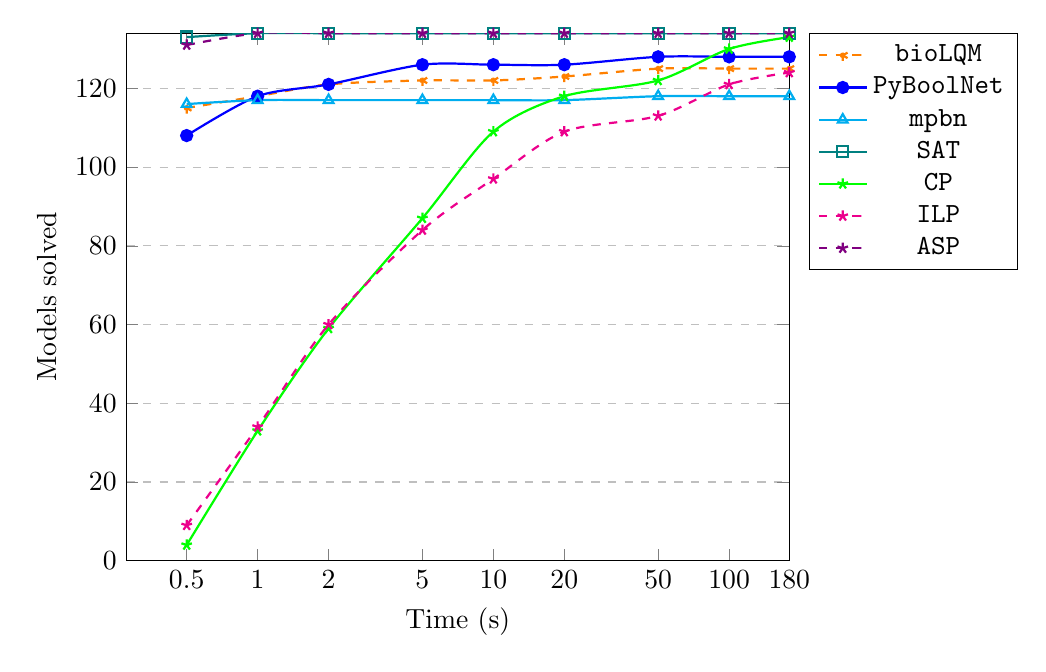
\begin{tikzpicture}
		\begin{semilogxaxis}[
			%title={},
			xlabel={Time (s)},
			ylabel={Models solved},
			xmin=-1, xmax=180,
			%xmode=log,
			%log basis x={10},
			%scale only axis,
			ymin=0, ymax=134,
			%ymode=log,
			%log basis y={2},
			xtick={0.5, 1, 2, 5, 10, 20, 50, 100, 180},
			xticklabels = {0.5, 1, 2, 5, 10, 20, 50, 100, 180},
			ytick={0,20,40,60,80,100,120},
			y=0.5cm/10,
			%legend style={font=\fontsize{7}{8}\selectfont},
			%legend style={at={(1.2,-0.1)},anchor=north west},
			legend pos=outer north east,
			ymajorgrids=true,
			grid style=dashed,
		]
		
		\addplot[
			smooth,
			thick,
			dashed,
			color=orange,
			mark=asterisk,
		]
		coordinates {
			(0.5, 115)(1, 118)(2, 121)(5, 122)(10, 122)(20, 123)(50, 125)(100, 125)(180, 125)
		}; \addlegendentry{\texttt{bioLQM}}
		
		\addplot[
			smooth,
			thick,
			color=blue,
			mark=*,
		]
		coordinates {
			(0.5, 108)(1, 118)(2, 121)(5, 126)(10, 126)(20, 126)(50, 128)(100, 128)(180, 128)
		}; \addlegendentry{\texttt{PyBoolNet}}
		
		\addplot[
			smooth,
			thick,
			%dashed,
			color=cyan,
			mark=triangle,
		]
		coordinates {
			(0.5, 116)(1, 117)(2, 117)(5, 117)(10, 117)(20, 117)(50, 118)(100, 118)(180, 118)
		}; \addlegendentry{\texttt{mpbn}}
		
		\addplot[
			smooth,
			thick,
			%dashed,
			color=teal,
			mark=square,
		]
		coordinates {
			(0.5, 133)(1, 134)(2, 134)(5, 134)(10, 134)(20, 134)(50, 134)(100, 134)(180, 134)
		}; \addlegendentry{\texttt{SAT}}
		
		\addplot[
			smooth,
			thick,
			%dashed,
			color=green,
			mark=star,
		]
		coordinates {
			(0.5, 4)(1, 33)(2, 59)(5, 87)(10, 109)(20, 118)(50, 122)(100, 130)(180, 133)
		}; \addlegendentry{\texttt{CP}}
		
		
		\addplot[
			smooth,
			thick,
			dashed,
			color=magenta,
			mark=star,
		]
		coordinates {
			(0.5, 9)(1, 34)(2, 60)(5, 84)(10, 97)(20, 109)(50, 113)(100, 121)(180, 124)
		}; \addlegendentry{\texttt{ILP}}
		
		\addplot[
			smooth,
			thick,
			dashed,
			color=violet,
			mark=star,
		]
		coordinates {
			(0.5, 131)(1, 134)(2, 134)(5, 134)(10, 134)(20, 134)(50, 134)(100, 134)(180, 134)
		}; \addlegendentry{\texttt{ASP}}
		
		\end{semilogxaxis}
	\end{tikzpicture}
	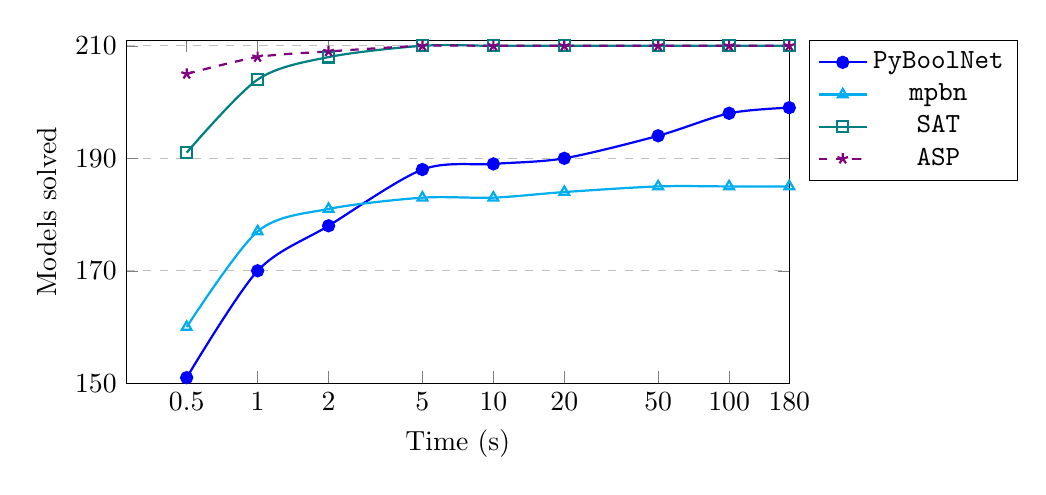
\begin{tikzpicture}
		\begin{semilogxaxis}[
			%title={},
			xlabel={Time (s)},
			ylabel={Models solved},
			xmin=-1, xmax=180,
			log basis x={10},
			%scale only axis,
			ymin=150, ymax=211,
			%ymode=log,
			%log basis y={10},
			xtick={0.5, 1, 2, 5, 10, 20, 50, 100, 180},
			xticklabels = {0.5, 1, 2, 5, 10, 20, 50, 100, 180},
			ytick={150, 170, 190, 210},
			y=0.5cm/7,
			%legend style={font=\fontsize{7}{8}\selectfont},
			%legend style={at={(0.0,-0.1)},anchor=north},
			legend pos=outer north east,
			ymajorgrids=true,
			grid style=dashed,
		]
	
		\addplot[
			smooth,
			thick,
			color=blue,
			mark=*,
		]
		coordinates {
			(0.5, 151)(1, 170)(2, 178)(5, 188)(10, 189)(20, 190)(50, 194)(100, 198)(180, 199)
		}; \addlegendentry{\texttt{PyBoolNet}}
		
		\addplot[
			smooth,
			thick,
			%dashed,
			color=cyan,
			mark=triangle,
		]
		coordinates {
			(0.5, 160)(1, 177)(2, 181)(5, 183)(10, 183)(20, 184)(50, 185)(100, 185)(180, 185)
		}; \addlegendentry{\texttt{mpbn}}
		
		\addplot[
			smooth,
			thick,
			%dashed,
			color=teal,
			mark=square,
		]
		coordinates {
			(0.5, 191)(1, 204)(2, 208)(5, 210)(10, 210)(20, 210)(50, 210)(100, 210)(180, 210)
		}; \addlegendentry{\texttt{SAT}}
		
%		\addplot[
%			smooth,
%			thick,
%			%dashed,
%			color=green,
%			mark=star,
%		]
%		coordinates {
%			(0.5, 4)(1, 33)(2, 59)(5, 87)(10, 109)(20, 118)(50, 122)(100, 130)(180, 133)
%		}; \addlegendentry{\texttt{CP}}
		
		
		%		\addplot[
		%			smooth,
		%			thick,
		%			dashed,
		%			color=magenta,
		%			mark=star,
		%		]
		%		coordinates {
		%			(0.5, 9)(1, 34)(2, 60)(5, 84)(10, 97)(20, 109)(50, 113)(100, 121)(180, 124)
		%		}; \addlegendentry{\texttt{ILP}}
		
		\addplot[
			smooth,
			thick,
			dashed,
			color=violet,
			mark=star,
		]
		coordinates {
			(0.5, 205)(1, 208)(2, 209)(5, 210)(10, 210)(20, 210)(50, 210)(100, 210)(180, 210)
		}; \addlegendentry{\texttt{ASP}}
	
	\end{semilogxaxis}
	\end{tikzpicture}
	\caption{Cumulative numbers of the \texttt{BBM} models that have less than 1000 minimal trap spaces (upper panel) and \texttt{BBM} models solved by the compared methods with respect to enumerating the first 1000 minimal trap spaces (lower panel).}
	\label{fig:BBM_cumul}
\end{figure}


Figure~\ref{fig:BBM_cumul} (upper panel) shows cumulative numbers of the \texttt{BBM} models that have less than 1000 minimal trap spaces solved by the compared methods with respect to enumerating the first 1000 minimal trap spaces.
The number of such models is 134 (per all 211 models), and 15 of them are non-locally-monotonic.
This model set allows us to fairly consider \texttt{bioLQM} for comparison, since \texttt{bioLQM} always requires to compute all minimal trap spaces.
We can first see that \texttt{Trappist-ASP} and \texttt{Trappist-MaxSAT} are still the two best methods as they can handle every model within 1s as well as they always can handle more models than all the remaining methods on every time limit.
Second, \texttt{Trappist-CP} is better than \texttt{Trappist-ILP}, which is consistent with their comparison shown in the previous subsection.
Third, one notable remark is that for the time limit of 100s or 180s, \texttt{Trappist-CP} can handle more models than all \texttt{bioLQM}, \texttt{PyBoolNet}, and \texttt{mpbn}.
This remark shows that even with a not best implementation, our alternative approach is still better than the state-of-the-art methods on a certain set of real-world models.
This is supported by the fact that our alternative approach avoids the need for computing prime implicants (as opposed to \texttt{PyBoolNet}) and can handle non-locally-monotonic Boolean networks (as opposed to \texttt{mpbn}).


Figure~\ref{fig:BBM_cumul} (lower panel) shows cumulative numbers of the \texttt{BBM} models solved by the compared methods (except \texttt{bioLQM}, \texttt{Trappist-CP}, and \texttt{Trappist-ILP}) with respect to enumerating the first 1000 minimal trap spaces.
We omit the results of \texttt{Trappist-CP} and \texttt{Trappist-ILP} because they can handle no model with more than 1000 minimal trap spaces.
Again, we can see that \texttt{Trappist-ASP} and \texttt{Trappist-MaxSAT} are the two best methods as they can handle every but one model within 5s. They also always handle many more models than both \texttt{PyBoolNet} and \texttt{mpbn} on every time limit.
Note that with the time limit of 0.5s, \texttt{Trappist-ASP} can handle 14 more models than \texttt{Trappist-MaxSAT}, which is opposed to the case of models with less than 1000 minimal trap spaces (see Figure~\ref{fig:BBM_cumul} (upper panel)).
This observation confirms the disadvantage of \texttt{Trappist-MaxSAT} compared to \texttt{Trappist-ASP} for the case of many minimal trap spaces.


\subsection{Selected models}
\label{subsec:Selected_models}

We used a set of real-world Boolean networks lying in various scales collected from numerous bibliographic sources in the literature.
Most of these models are quite big (in size), complex (i.e., having high average in-degree, which is related to the number of prime-implicants), and have never been fully analyzed.
Note that these models are not included in the \texttt{PyBoolNet} and \texttt{BBM} repositories.
We then applied \texttt{bioLQM}, \texttt{PyBoolNet}, \texttt{mpbn}, and the four variants of \texttt{Trappist} to computing minimal trap spaces of these real-world models.
Table~\ref{tab:result_real} shows the obtained experimental results.
A number in bold indicates a ratio greater than or equal to 10 compared to the best result.
The remaining notations are similar to those in Table~\ref{tab:pyboolnet_repo}.
Hereafter, we analyze in detail the results with respect to minimal trap space computation.

\begin{table}[!htb]
  \caption{Timing comparisons (in seconds) between \texttt{bioLQM} (\texttt{LQM}), \texttt{PyBoolNet} (\texttt{PBN}), \texttt{mpbn} and the four variants of \texttt{Trappist} on selected models from the literature.}
  % in bold if greater than or equal to 10
  \centering%
  \label{tab:result_real}
  \scalebox{0.76}{
  \begin{tabular}{rlrrrrrrrrr}
    \toprule
    & & & & & & & \multicolumn{4}{c}{\texttt{Trappist}}\\
    \cmidrule(rr){8-11}
    & model & \(n\) & \(|M|\) & \texttt{LQM} & \texttt{PBN} & \texttt{mpbn} & \texttt{SAT} & \texttt{CP} & \texttt{ILP} & \texttt{ASP} \\
    \midrule % n < 100
    \rownb & metastatic~\cite{DesignPrinciplesGeneNetworks} & 10 & 4 & \textbf{0.10} & 0.04 & NM & 0.01 & \textbf{1.15} & \textbf{0.89} & 0.02 \\
    \rownb & Arabidopsis\_thaliana~\cite{DesignPrinciplesGeneNetworks} & 15 & 8 & \textbf{0.10} & 0.06 & NM & 0.01 & \textbf{2.06} & \textbf{1.83} & 0.02 \\
    \rownb & p53\_high\_dna~\cite{DesignPrinciplesGeneNetworks} & 16 & 1 & 0.38 & \textbf{1.76} & NM & 0.08 & 0.53 & 0.43 & 0.14 \\
    \rownb & p53\_low\_dna~\cite{DesignPrinciplesGeneNetworks} & 16 & 1 & 0.41 & \textbf{1.76} & NM & 0.07 & 0.58 & 0.48 & 0.14 \\
    \rownb & FT-GRN~\cite{ChvezHernndez2022} & 23 & 32 & \textbf{DNF} & \textbf{DNF} & NM & 0.03 & \textbf{8.41} & \textbf{12.38} & 0.19 \\
    \rownb & DNA\_damage~\cite{DesignPrinciplesGeneNetworks} & 26 & 16 & \textbf{0.24} & \textbf{0.33} & NM & 0.02 & \textbf{3.91} & \textbf{5.33} & 0.05 \\
    \rownb & Rho-GTPases~\cite{DesignPrinciplesGeneNetworks} & 33 & 2 & 0.17 & 0.57 & \textbf{40.39} & 0.07 & \textbf{0.74} & 0.56 & 0.11 \\
    \rownb & Pluripotency~\cite{YachieKinoshita2018} & 36 & 440 & \textbf{DNF} & \textbf{DNF} & NM & 0.16 & \textbf{138.92} & \textbf{DNF} & 0.28 \\
    \rownb & Pluripotent~\cite{DesignPrinciplesGeneNetworks} & 36 & 276 & 0.37 & 0.43 & NM & 0.07 & \textbf{72.40} & \textbf{DNF} & 0.06 \\
    \rownb & Pancreatic\_Cancer~\cite{DesignPrinciplesGeneNetworks} & 43 & $1000^+$ & N/A & 0.11 & 0.36 & 0.17 & \textbf{DNF} & \textbf{DNF} & 0.06 \\
    \rownb & Drosophila~\cite{RodrguezVega2014} & 52 & 128 & 0.33 & 0.05 & 0.07 & 0.06 & \textbf{32.66} & \textbf{126.22} & 0.05 \\
    \rownb & Cacace\_TdevModel~\cite{Cacace2020} & 61 & 28 & \textbf{1.29} & \textbf{5.67} & NM & 0.06 & \textbf{7.51} & \textbf{23.15} & 0.08 \\
    \rownb & hedgehog~\cite{DesignPrinciplesGeneNetworks} & 65 & $1000^+$ & N/A & \textbf{DNF} & 0.50 & 0.34 & \textbf{DNF} & \textbf{DNF} & 0.33 \\
    \rownb & EMT~\cite{Rozum2021} & 69 & 268 & \textbf{39.22} & \textbf{1.01} & 0.20 & 0.12 & \textbf{75.81} & \textbf{DNF} & 0.05 \\
    \rownb & Bcell~\cite{Dutta2019} & 73 & 72 & 0.23 & 0.04 & 0.08 & 0.06 & \textbf{18.95} & \textbf{81.85} & 0.05 \\
    \rownb & mast\_cell~\cite{aghamiri2020automated} & 73 & $1000^+$ & N/A & 0.09 & 0.55 & 0.37 & \textbf{DNF} & \textbf{DNF} & 0.15 \\
    \rownb & Corral\_ThIL17diff~\cite{corral2021interplay} & 92 & $1000^+$ & N/A & \textbf{107.57} & 0.76 & 0.56 & \textbf{DNF} & \textbf{DNF} & 0.16 \\

    \midrule % 100 <= n < 200
     \rownb & Adhesion\_CIP~\cite{guberman2020boolean} & 121 & 78 & \textbf{56.81} & \textbf{4.25} & 0.23 & 0.17 & \textbf{25.20} & \textbf{DNF} & 0.19 \\
    \rownb & EMT\_Mech~\cite{Sullivan2022} & 136 & 82 & \textbf{DNF} & \textbf{14.01} & 0.27 & 0.20 & \textbf{27.55} & \textbf{DNF} & 0.25 \\
    \rownb & macrophage~\cite{DesignPrinciplesGeneNetworks} & 136 & $1000^+$ & N/A & 0.54 & 1.09 & 0.84 & \textbf{DNF} & \textbf{DNF} & 0.27 \\
    \rownb & angiogenesis~\cite{DesignPrinciplesGeneNetworks} & 141 & $1000^+$ & N/A & 0.16 & 1.07 & 1.06 & \textbf{DNF} & \textbf{DNF} & 0.16 \\
    \rownb & angiofull~\cite{Weinstein2017} & 142 & $1000^+$ & N/A & 0.17 & 1.06 & 0.88 & \textbf{DNF} & \textbf{DNF} & 0.23 \\
    \rownb & EMT\_Mech\_TGFbeta~\cite{Sullivan2022} & 150 & 492 & \textbf{DNF} & \textbf{11.28} & 0.78 & 0.69 & \textbf{DNF} & \textbf{DNF} & 0.35 \\
    \rownb & RA\_apoptosis~\cite{aghamiri2020automated} & 180 & $1000^+$ & N/A & \textbf{DNF} & 1.43 & 1.55 & \textbf{DNF} & \textbf{DNF} & 0.19 \\
    \rownb & MAPK~\cite{aghamiri2020automated} & 181 & $1000^+$ & N/A & \textbf{13.58} & 1.76 & 1.51 & \textbf{DNF} & \textbf{DNF} & 0.27 \\

    \midrule % 200 <= n
    \rownb & Snf1-pathway~\cite{Lubitz2015} & 202 & $1000^+$ & N/A & 1.13 & 1.47 & 1.43 & \textbf{DNF} & \textbf{DNF} & 0.31 \\
    \rownb & T-cell-co-receptor~\cite{DesignPrinciplesGeneNetworks} & 206 & $1000^+$ & N/A & \textbf{DNF} & 1.52 & 2.26 & \textbf{DNF} & \textbf{DNF} & 0.35 \\
    \rownb & TcellCheckPoint~\cite{hernandez2020computational} & 218 & $1000^+$ & N/A & \textbf{4.99} & NM & 1.96 & \textbf{DNF} & \textbf{DNF} & 0.28 \\
    \rownb & Mycobacterium~\cite{DesignPrinciplesGeneNetworks} & 317 & $1000^+$ & N/A & 0.42 & 2.36 & \textbf{4.91} & \textbf{DNF} & \textbf{DNF} & 0.44 \\
    \rownb & Leishmania~\cite{DesignPrinciplesGeneNetworks} & 342 & $1000^+$ & N/A & \textbf{DNF} & 2.56 & \textbf{5.62} & \textbf{DNF} & \textbf{DNF} & 0.46 \\
    \rownb & Cholocystokinin~\cite{aghamiri2020automated} & 383 & $1000^+$ & N/A & 0.36 & 2.99 & \textbf{4.81} & \textbf{DNF} & \textbf{DNF} & 0.37 \\
    \rownb & Alzheimer~\cite{aghamiri2020automated} & 762 & $1000^+$ & N/A & \textbf{DNF} & NM & \textbf{18.21} & \textbf{DNF} & \textbf{DNF} & 0.79 \\

    \bottomrule
  \end{tabular}
  }
\end{table}

First, we obtained some observations on the four variants of \texttt{Trappist} consistent with the observations obtained in the previous subsections.
More specifically, \texttt{Trappist-ASP} is still the best variant with a running time below one second for every model, and followed by \texttt{Trappist-MaxSAT}.
In particular, the difference in running time between \texttt{Trappist-ASP} and \texttt{Trappist-MaxSAT} is bigger for larger models or models with more than 1000 minimal trap spaces.
\texttt{Trappist-CP} and \texttt{Trappist-ILP} still have a much worse performance, with \texttt{Trappist-CP} better than \texttt{Trappist-ILP}.
They still can handle no model with more than 1000 minimal trap spaces.
However, \texttt{Trappist-CP} or \texttt{Trappist-ILP} can handle the FT-GRN and Pluripotency models, whereas all \texttt{bioLQM}, \texttt{PyBoolNet}, and \texttt{mpbn} cannot.

Second, \texttt{Trappist-ASP} (even \texttt{Trappist-MaxSAT}) is far more efficient than both \texttt{bioLQM} and \texttt{PyBoolNet} on every model where the comparison is possible.
For most models, the speedups of \texttt{Trappist-ASP} compared to \texttt{bioLQM} and \texttt{PyBoolNet} are between one and three orders of magnitude.
This again confirms the superiority of \texttt{Trappist-ASP} compared to the other methods that can handle general Boolean networks.

Third, for 11 of the 32 models (more than 34\%), \texttt{mpbn} did not give any answer because these models are non-locally-monotonic.
For 21 of the 32 models where \texttt{mpbn} returned the answers, \texttt{mpbn} and \texttt{Trappist-ASP} are roughly comparable in computation time, but \texttt{mpbn} appears quite slower on average.
In particular, for the Rho-GTPases model, \texttt{mpbn} is \(577\times\) slower than \texttt{Trappist-ASP}.
This observation along with the comparisons between \texttt{mpbn} and \texttt{Trappist-ASP} in the previous subsections are quite surprising because the ASP encoding of \texttt{mpbn} only requires the DNF for the activation part of a Boolean function, whereas that of \texttt{Trappist-ASP} requires both the activation and inhibition parts (see Subsection~\ref{subsec:computation_asp}).
However, the reason may lie on the differences in the ASP encoding characteristics of the two methods and the fact that \texttt{mpbn} needs to spend time checking the local-monotonicity of each Boolean function in a Boolean network.
We expect that \texttt{mpbn} may outperform \texttt{Trappist} for a certain set of models, but not for the set of real-world models considered in this article.

Fourth, regarding the comparison of the ASP-based methods (i.e., \texttt{PyBoolNet}, \texttt{mpbn}, and \texttt{Trappist-ASP}), we note that for all the models where \texttt{PyBoolNet} did not finish before the time limit, the timeout occurred during the computation of the prime-implicants.
Hence, not even a single minimal trap space was output by that method.
For all the remaining models, once \texttt{PyBoolNet} went through the prime-implicant phase, its ASP solving phase quickly returned the first 1000 minimal trap spaces, all under one second.
Hence, with the experimental results shown in this subsection as well as the two previous subsections, the practical differences between the ASP encoding of \texttt{Trappist-ASP} and that of \texttt{PyBoolNet} are not distinctly exposed.
The fact that our new ASP encoding is guaranteed to be linear in the number of nodes of the original model (see Subsection~\ref{subsec:computation_asp}) does not seem to be crucial here, however a much deeper analysis of those cases shall be shown in the next subsection.

%The second observation is that the proposed method vastly outperforms \texttt{PyBoolNet} in computational time, on each and every model, and sometimes with orders of magnitude of difference (e.g., for most models in the 100--1000 nodes size range).
%Note that for all the cases where \texttt{PyBoolNet} did not manage to finish before the timeout, as marked by ``DNF'' in Table~\ref{tab:result_real}, the timeout occurred during the computation of the prime-implicants.
%Hence, not even a single minimal trap space was output by that method.
%The computational advantage is therefore immediately a practical advantage since on the one hand the state-of-the-art method did not allow any analysis whatsoever of the models, and on the other hand the proposed method could provide, very often under one second, the first thousand minimal trap spaces.
%For modellers having a critical look at a model and in a \emph{model, invalidate, refine} loop this means a huge difference in the models that are amenable to study.
%
%Note that even with a very restricted time-limit of two minutes, it was possible with the proposed technique to find \emph{all} minimal trap spaces of small models (roughly under 130 nodes, i.e., considered as quite big up to now).
%Though it might seem impractical to handle tens of thousands of such possible complex attractors in a manual way, i.e., to compare them to specific experimental conditions and corresponding data, we hope that an automatic analysis of such attractors might become possible with systematic verification methods, not unlike that described in~\cite{hernandez2020computational}.
%Since the ASP code is declarative by nature, it is also possible to add to it supplementary constraints coming from the modeler in case one is looking for specific attractors.
%Finally, sampling from the ASP-generated solutions as is done in~\cite{chevalier2020synthesis} would allow for a different type of exploration.
%
%The third observation is that for all the models where \texttt{PyBoolNet} finished before the timeout, once \texttt{PyBoolNet} went through the prime-implicant phase, its ASP solving phase quickly returned the first 1000 minimal trap spaces, all under one second.
%For these models, the ASP solving phase of the proposed method also took very short time, all under one second.
%Hence, with the experimental results shown in this paper, the practical differences between our ASP encoding and that of \texttt{PyBoolNet} are not distinctly exposed.
%The fact that our new ASP encoding is guaranteed to be linear in the number of nodes of the original model does not seem to be crucial here, however a much deeper analysis of those cases remains to be done.
%
%Note that though enumerating the extremal siphons of a Petri net is exponential (see~\cite{nabli2016enumerating} for instance) this is apparently not the bottleneck of the proposed method, showing once again that networks obtained from biochemical models do have a specific structure.

\subsection{Randomly generated models}

We randomly generated a set of N-K models~\cite{glass1973logical} with network size \(n\) in the set \{100, 150, 200, 250, 300, 350, 400\} and in-degree \(K = 3\) (i.e., each node has exactly three input nodes).
We chose N-K models because they are a useful tool for studying the dynamics of Boolean networks~\cite{glass1973logical,klarner2015computing,Rozum2021}.
For each network size, 50 instances were generated using the \verb|generateRandomNKNetwork| function.
In total, we have 350 random models.
We then applied the compared methods to these models and recorded the running time of each method for each model.
It is worth noting that N-K models usually have small numbers of minimal trap spaces~\cite{klarner2015computing}.
Hence, we searched for all solutions in each model, which makes the comparison to \texttt{bioLQM} more comprehensive.
In addition, each node has only three input nodes, leading to the number of prime-implicants of the associated Boolean function is small.
Hence, \texttt{PyBoolNet} always passed the phase of computing prime-implicants in every model even within one second, which enables us to compare the ASP encoding of \texttt{PyBoolNet} and that of \texttt{Trappist-ASP}.

\begin{figure}[!ht]
	\centering
	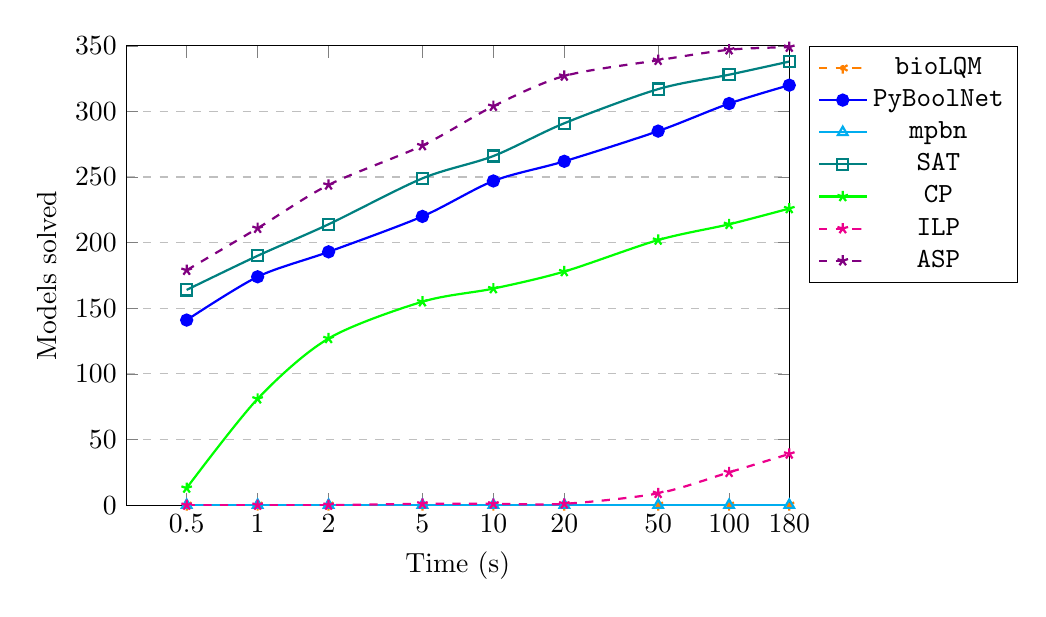
\begin{tikzpicture}
	\begin{semilogxaxis}[
		%title={},
		xlabel={Time (s)},
		ylabel={Models solved},
		xmin=-1, xmax=180,
		log basis x={10},
		%scale only axis,
		ymin=0, ymax=350,
		%ymode=log,
		%log basis y={10},
		xtick={0.5, 1, 2, 5, 10, 20, 50, 100, 180},
		xticklabels = {0.5, 1, 2, 5, 10, 20, 50, 100, 180},
		ytick={0, 50, 100, 150, 200, 250, 300, 350},
		y=0.5cm/30,
		%legend style={font=\fontsize{7}{8}\selectfont},
		%legend style={at={(0.0,-0.1)},anchor=north},
		legend pos=outer north east,
		ymajorgrids=true,
		grid style=dashed,
	]
	
	\addplot[
		smooth,
		thick,
		dashed,
		color=orange,
		mark=asterisk,
	]
	coordinates {
		(0.5, 0)(1, 0)(2, 0)(5, 0)(10, 0)(20, 0)(50, 0)(100, 0)(180, 0)
	}; \addlegendentry{\texttt{bioLQM}}
	
	\addplot[
		smooth,
		thick,
		color=blue,
		mark=*,
	]
	coordinates {
		(0.5, 141)(1, 174)(2, 193)(5, 220)(10, 247)(20, 262)(50, 285)(100, 306)(180, 320)
	}; \addlegendentry{\texttt{PyBoolNet}}
	
	\addplot[
		smooth,
		thick,
		%dashed,
		color=cyan,
		mark=triangle,
	]
	coordinates {
		(0.5, 0)(1, 0)(2, 0)(5, 0)(10, 0)(20, 0)(50, 0)(100, 0)(180, 0)
	}; \addlegendentry{\texttt{mpbn}}
	
	\addplot[
		smooth,
		thick,
		%dashed,
		color=teal,
		mark=square,
	]
	coordinates {
		(0.5, 164)(1, 190)(2, 214)(5, 249)(10, 266)(20, 291)(50, 317)(100, 328)(180, 338)
	}; \addlegendentry{\texttt{SAT}}

	\addplot[
		smooth,
		thick,
		%dashed,
		color=green,
		mark=star,
	]
	coordinates {
		(0.5, 13)(1, 81)(2, 127)(5, 155)(10, 165)(20, 178)(50, 202)(100, 214)(180, 226)
	}; \addlegendentry{\texttt{CP}}


	\addplot[
		smooth,
		thick,
		dashed,
		color=magenta,
		mark=star,
	]
	coordinates {
		(0.5, 0)(1, 0)(2, 0)(5, 1)(10, 1)(20, 1)(50, 9)(100, 25)(180, 39)
	}; \addlegendentry{\texttt{ILP}}
	
	\addplot[
		smooth,
		thick,
		dashed,
		color=violet,
		mark=star,
	]
	coordinates {
		(0.5, 179)(1, 211)(2, 244)(5, 274)(10, 304)(20, 327)(50, 339)(100, 347)(180, 349)
	}; \addlegendentry{\texttt{ASP}}

	\end{semilogxaxis}
	\end{tikzpicture}
	\caption{Cumulative numbers of random models solved by the compared methods with respect to enumerating all the minimal trap spaces.}
	\label{fig:random_cumul_first}
\end{figure}

%\begin{table}[!htb]
%  \caption{Results on N-K models.}
%  \centering%
%  \label{tab:result_N_K}
%  \begin{tabular}{rrrrrrrr}
%    \toprule
%    & & & & \multicolumn{4}{c}{\texttt{Trappist}}\\
%    \cmidrule(rr){5-8}
%    \(n\) & \texttt{LQM} & \texttt{mpbn} & \texttt{PBN} & \texttt{SAT} & \texttt{CP} & \texttt{ILP} & \texttt{ASP} \\
%    \midrule
%    100 & 50 ($>$ 180) & 50 (N/A) & 0 (0.07) & 0 (0.05) & - () & - () & 0 (0.09) \\
%    150 & 50 ($>$ 180) & 50 (N/A) & 0 (0.14) & 0 (0.10) & - () & - () & 0 (0.14) \\
%    200 & 50 ($>$ 180) & 50 (N/A) & 0 (0.43) & 0 (0.25) & - () & - () & 0 (0.24) \\
%    250 & 50 ($>$ 180) & 50 (N/A) & 0 (1.92) & 0 (1.04) & - () & - () & 0 (0.56) \\
%    300 & 50 ($>$ 180) & 50 (N/A) & 0 (9.68) & 0 (4.46) & - () & - () & 0 (1.83) \\
%    350 & 50 ($>$ 180) & 50 (N/A) & 1 (46.54) & 0 (20.09) & - () & - () & 0 (6.10) \\
%    400 & 50 ($>$ 180) & 50 (N/A) & 29 (144.09) & 12 (90.36) & - () & - () & 1 (33.01) \\
%    \bottomrule
%  \end{tabular}
%\end{table}

%Table~\ref{tab:result_N_K} shows the experimental results on N-K models.
%Column \(n\) denotes the network size.
%Columns \texttt{LQM} and \texttt{PBN} show the results of \texttt{bioLQM} and \texttt{PyBoolNet}, respectively.
%For each method, the number outside the parentheses indicates the number of failures, whereas the number inside the parentheses indicates the average running time (in seconds).
%Note that when computing the average running time, if the running time exceeds 180s, it is considered as 180s.
%From these results, we obtained several observations consistent with those obtained for real-world models.

Figure~\ref{fig:random_cumul_first} shows cumulative numbers of random models solved by the compared methods with respect to enumerating all the minimal trap spaces.
The number of succeeded models within three minutes for each method is: \texttt{bioLQM} (0), \texttt{PyBoolNet} (320), \texttt{mpbn} (0), \texttt{Trappist-maxSAT} (338), \texttt{Trappist-CP} (226), \texttt{Trappist-ILP} (39), \texttt{Trappist-ASP} (349).
We can see that \texttt{Trappist-ASP} is the only method that can handle every model, but one.
Note that none of the other methods can handle that only model failed by \texttt{Trappist-ASP}.
We also obtained some observations consistent with those obtained for real-world models.
More specifically, \texttt{Trappist-MaxSAT} is still the second best method and \texttt{Trappist-CP} is better than \texttt{Trappist-ILP}.
Upon closer inspection, we obtained several notable observations as follows.

First, \texttt{mpbn} was not able to handle any model because all the models are non-locally-monotonic.
Recall that a Boolean network is non-locally-monotonic if only one of its Boolean functions is non-locally-monotonic.
Hence, it is apparent that all this type of randomly generated models are non-locally-monotonic because of the number of nodes is large (\(n \geq 100\)).
This observation confirms a limit on the applicable model class of \texttt{mpbn}.

Second, surprisingly \texttt{bioLQM} cannot handle any model.
One of the reason may be that the BDD characterizing all trap spaces is too large, and its computation is slow.
In addition, having too many generic trap spaces before the filtering process may be also a reason.
It is apparent because the network size is large (\(n \geq 100\)) and the Boolean functions are not simple.

Third, for every time limit, \texttt{Trappist-ASP} can always handle many more models than \texttt{PyBoolNet}, ranging from 29 to 65 more models.
Since the time for the phase of computing prime-implicants of \texttt{PyBoolNet} is negligible in every model, most of the running time of \texttt{PyBoolNet} was spent for its ASP solving phase.
Hence, we can easily see that the ASP encoding of \texttt{Trappist-ASP} is much better than that of \texttt{PyBoolNet}. 
This observation is consistent with the theoretical comparison in the ASP encoding between \texttt{Trappist-ASP} and \texttt{PyBoolNet} mentioned in Subsection~\ref{subsec:computation_asp}.

%More models handled by Trappist-ASP: 38, 37, 51, 54, 57, 65, 54, 41, 29

\subsection{Experimental summary}
\label{subsec:Experimental_summary}

We have tested our alternative approach on many Boolean network models of various sizes and types (e.g., real-world models, randomly generated models) on existing and newly created benchmarks.
This indicates the high coverage and comprehensiveness of the experiments.

Among the four variants of the alternative approach, \texttt{Trappist-ASP} is the best method as it vastly outperforms all the other variants.
The second best one is \texttt{Trappist-MaxSAT}.
The two remaining variants (i.e., \texttt{Trappist-CP} and \texttt{Trappist-ILP}) give bad performance for most models.
However, for certain cases, they are still better than all state-of-the-art methods (i.e., \texttt{bioLQM}, \texttt{PyBoolNet}, and \texttt{mpbn}).
This is evidence for the advantages of an alternative approach compared to what preexisted.

Regarding general Boolean networks, \texttt{Trappist-ASP} (even \texttt{Trappist-MaxSAT}) is far more efficient than both \texttt{bioLQM} and \texttt{PyBoolNet}.
The speedups of \texttt{Trappist-ASP} or \texttt{Trappist-MaxSAT} are large, even between one and three orders of magnitude for most models.
In addition, the experimental results also confirm that the ASP encoding of \texttt{Trappist-ASP} is much more efficient than that of \texttt{PyBoolNet}.

Regarding locally-monotonic Boolean networks, the performance of \texttt{mpbn} is roughly comparable to that of \texttt{Trappist-ASP} or \texttt{Trappist-MaxSAT}.
However, \texttt{mpbn} is quite slower than \texttt{Trappist-ASP} on average.
This shows the practical advantage of \texttt{Trappist-ASP} compared to \texttt{mpbn}, though its ASP encoding may be more complex than that of \texttt{mpbn} in theory.


\section{Conclusion}%
\label{sec:Conclusion}

In this article we have explored and proved for the first time the equivalence between (minimal) trap spaces of a general Boolean network and (maximal) conflict-free siphons of its Petri net encoding.
We have shown several useful applications of this finding to studying properties of trap spaces in Boolean networks.
As an important practical application of the equivalence, we have proposed a new approach for the computation of minimal trap spaces in Boolean networks, based on the enumeration of maximal conflict-free siphons of Petri nets.
We have also proposed four possible methods using MaxSAT, CP, ILP, and ASP for implementing the new approach.
In particular, we have shown how to adjust our approach to compute several specific types of trap spaces (e.g., maximal trap spaces, fixed points), which besides minimal trap spaces also play crucial roles in the analysis and control of Boolean networks.
The proposed methods for the minimal trap space computation have been evaluated on many real-world models from the literature as well as randomly generated models.
The experimental results show that the new approach vastly outperforms all the state-of-the-art methods in terms of general Boolean networks and is comparable to the \texttt{mpbn} method even much better on average in terms of locally-monotonic Boolean networks.
We believe that this opens up the way to a much better analysis of large Boolean networks, which is needed with the advent of automatic model-generation pipelines~\cite{ostaszewski2021covid19}.

Although the experimental results show the superiority of our approach to \texttt{mpbn} in general, we however note that there is a model in the \texttt{BBM} repository (with identifier 122) where all the four proposed methods for the new approach did not manage to finish the Petri net conversion before the timeout, whereas \texttt{mpbn} can still handle this model.
The model is not very large but its Boolean functions are rather complicated.
This points to the fact that our current choice of using a BDD-based translation to obtain that Petri net encoding, though it provides a small/efficient ASP might be too costly to handle the complex models.
In such a case, a more \emph{naive} encoding might provide a much larger ASP program, with many redundant rules, but easier/faster to obtain.
The evaluation of the feasibility of such strategy, and of its impact on smaller instances, remains to be done.
Recognizing that a model is locally-monotonic and applying in that specific case dedicated strategies as those of \texttt{mpbn} might also be a partial solution.

It is worth noting that there may be possibly other methods for computing minimal/maximal conflict-free siphons in Petri nets, like the methods for generic siphon computation in the field of Petri nets (see~\cite{DBLP:journals/isci/LiuB16} for a survey about these methods).
Although these approaches do not directly support the minimal/maximal conflict-free siphon computation now, we plan to investigate them in the future.
They could replace our proposed methods if they give significantly better performance.
However, the current methods appear to already perform very well even on the biggest models we have considered.

Finally, we think that the links between Petri nets and Boolean networks that we stumbled upon in this article might have deeper roots.
Exploring those connections might lead both to interesting topics of research for Petri nets, like a notion of trap-spaces, and for Boolean networks.
We also believe that the connection between trap spaces of Boolean networks and siphons of Petri nets can be a very useful tool for exploring and proving more new properties of trap spaces in Boolean networks, as we have used it to successfully prove the independence of trap spaces to the update scheme and the separation of minimal trap spaces.
Diving into this direction is promising and one of our future work.


%% The Appendices part is started with the command \appendix;
%% appendix sections are then done as normal sections
%% \appendix

%% \section{}
%% \label{}

%% For citations use:
%%       \citet{<label>} ==> Jones et al. [21]
%%       \citep{<label>} ==> [21]
%%

%% If you have bibdatabase file and want bibtex to generate the
%% bibitems, please use
%%
\bibliographystyle{elsarticle-num-names}
\bibliography{tcs2023.bib}

%% else use the following coding to input the bibitems directly in the
%% TeX file.

% \begin{thebibliography}{00}

% %% \bibitem[Author(year)]{label}
% %% Text of bibliographic item

% \bibitem[ ()]{}

% \end{thebibliography}
\end{document}

\endinput
%%
%% End of file `elsarticle-template-num-names.tex'.
